\chapter{Обобщенная модель Изинга на одномерной цепочке при учете магнитного поля}\label{ch:ch2}

Начнем исследование модели Изинга с одномерного случая, поскольку он не представляет существенных вычислительных трудностей и в данном рассмотрении имеется возможность получения точных аналитических решений модели Изинга в присутствии магнитного поля.

\section{Обобщение модели Изинга на произвольное число трансляций линейной цепочки}\label{sec:ch2/sec1}

Гамильтониан обобщенной модели Изинга с произвольным числом обменных взаимодействий между ближайшими и вторыми соседями~\cite{kassan-ogly2001, dobson1969} линейной цепочки, находящейся в магнитном поле, может быть записан в следующей форме
\begin{multline}
\mathcal{H}_n(s)=-J_1\sum_{i=1,n+1,2n+1,\dots}^{N-n+1} s_i s_{i+1} - J_1^{'}\sum_{i=1,n+1,2n+1,\dots}^{N-n+1} s_i s_{i+2} -\\-J_2\sum_{i=2,n+2,2n+2,\dots}^{N-n+2} s_{i+1} s_{i+2} -J_2^{'}\sum_{i=2,n+2,2n+2,\dots}^{N-n+2} s_{i+1} s_{i+3} -\dots-\\ -J_n\sum_{i=n,2n,3n,\dots}^{N} s_{i+n} s_{i+n+1} - J_n^{'}\sum_{i=n,2n,3n,\dots}^{N} s_{i+n} s_{i+n+2} - H\sum_{i=1,2,3,\dots}^{N}s_i,
\label{1}
\end{multline}
где $J_1, J_2, \dots,  J_n$ --- параметры обменного взаимодействия между ближайшими соседями, $J^{'}_1, J^{'}_2, \dots, J^{'}_n$ --- параметры обменного взаимодействия между вторыми соседями, $H$ --- внешнее магнитное поле, $s=\pm 1$ (см. рисунок~\ref{6}, на котором представлен частный случай модели только с двумя различными обменами между ближайшими и вторыми соседями).

Следуя общему алгоритму вывода трансфер-матрицы Крамерса--Ваннье~\cite{kramers_wannier1}, можно получить трансфер-матрицы для одномерной цепочки с двумя, тремя, четырьмя и т.д. трансляциями в виде одной матрицы, например, для двух трансляций:
\begin{multline}
W_2=\\=
\begin{pmatrix}
e^{K_{1}+L_{1}+K_{2}+L_{2}+2h}\!\! &\! e^{K_{1}+L_{1}+K_{2}-L_{2}+2h}&\!\! e^{K_{1}-L_{1}-K_{2}+L_{2}+2h}\!\! &\! e^{K_{1}-L_{1}-K_{2}-L_{2}+2h}\\
e^{-K_{1}+L_{1}-K_{2}-L_{2}}\!\! &\! e^{-K_{1}+L_{1}-K_{2}+L_{2}}& \!\! e^{-K_{1}-L_{1}+K_{2}-L_{2}}\!\! &\! e^{-K_{1}-L_{1}+K_{2}+L_{2}}\\
e^{-K_{1}-L_{1}+K_{2}+L_{2}}\!\! &\!  e^{-K_{1}-L_{1}+K_{2}-L_{2}}&\!\! e^{-K_{1}+L_{1}-K_{2}+L_{2}}\!\!  &\!  e^{-K_{1}+L_{1}-K_{2}-L_{2}}\\
e^{K_{1}-L_{1}-K_{2}-L_{2}-2h}\!\! & \!  e^{K_{1}-L_{1}-K_{2}+L_{2}-2h}&\!\! e^{K_{1}+L_{1}+K_{2}-L_{2}-2h}\!\!  &\!   e^{K_{1}+L_{1}+K_{2}+L_{2}-2h}
\label{11}
\end{pmatrix}.
\end{multline}
где $K_1=J_1/T$, $K_2=J_2/T$, $L_1=J^{'}_1/T$, $L_2=J^{'}_2/T$, и $H=h/T$.

С другой стороны, перемножив две матрицы $V_1$ и $V_2$ каждая из которых соответствует одной трансляции, получаем в точности исходную матрицу $W_2$. Таким образом, показана эквивалентность $W_2$ и $V_1\cdot V_2$. Продолжая построение трансфер-матриц Крамерса-Ваннье для трех, четырех и т.д. трансляций в общем алгоритме вывода, будем получать все более и более громоздкие выражения, аналогичным образом превращаемые в гораздо более изящном виде в произведения простых матриц
\begin{multline}
W_n = V_1\cdot V_2 \cdot... \cdot V_n = \prod_{i=1}^n V_i =\\= \prod_{i=1}^n  \begin{pmatrix}
e^{K_{i}+L_{i}+h}\!\! &\! e^{K_{i}-L_{i}+h}&\!\! 0\!\! &\! 0\\
0\!\! &\! 0& \!\! e^{-K_{i}+L_{i}+h}\!\! &\! e^{-K_{i}-L_{i}+h}\\
e^{-K_{i}-L_{i}-h}\!\! &\!  e^{-K_{i}+L_{i}-h}&\!\! 0\!\!  &\!  0\\
0\!\! & \!  0&\!\! e^{K_{i}-L_{i}-h}\!\!  &\!   e^{K_{i}+L_{i}-h}\\
\end{pmatrix},
\label{2}
\end{multline}
где $V_1$, $V_2$, $\dots$, $V_n$ --- трансфер-матрицы Крамерса--Ваннье, \mbox{$K_i = J_i/T$}, \mbox{$L_i = J_i^{'}/T$}, $h=H/T$.

В результате трансфер-матрица Крамерса--Ваннье $W_n$ представляется как произведение трансфер-матриц $V_i$, относящихся к одной определенной трансляции линейной цепочки~[A1, A2, A3].

Поскольку в гамильтониане \eqref{1} каждая сумма пробегает только по $n$ узлам, а не по всем узлам решетки $N$, то статсумма в термодинамическом пределе теперь примет вид:
\begin{equation}
Z_N=\lambda_{\text{max}}^{N/n}.
\label{3}
\end{equation}

Свободная энергия, энтропия, теплоемкость, намагниченность и внутренняя энергия выражаются только через наибольшее собственное значение трансфер-матрицы Крамерса -- Ваннье $\lambda_{\text{max}}$
\begin{equation}
F(H,T)=-\frac{T \ln \lambda_{\text{max}}}{n},
\label{4}
\end{equation}
\begin{equation}
S(H,T)=\frac{\ln \lambda_{\text{max}}}{n}+\frac{T}{n\lambda_{\text{max}}}\frac{\partial \lambda_{\text{max}}}{\partial T},
\label{5}
\end{equation}
\begin{equation}
C(H,T)=\frac{T}{n\lambda_{\text{max}}}\frac{\partial \lambda_{\text{max}}}{\partial T} + \frac{T}{n}\frac{\partial }{\partial T}\bigg(\frac{T}{\lambda_{\text{max}}}\frac{\partial \lambda_{\text{max}}}{\partial T}\bigg),
\label{6}
\end{equation}
\begin{equation}
M(H,T)=\frac{T}{n\lambda_{\text{max}}}\frac{\partial \lambda_{\text{max}}}{\partial H},
\label{7}
\end{equation}
\begin{equation}
E(H,T)=\frac{T^2}{n}\frac{\partial \lambda_{\text{max}}}{\partial T}.
\label{8}
\end{equation}

Получение точного аналитического решения для наибольшего собственного значения трансфер-матрицы Крамерса--Ваннье с гамильтонианом \eqref{1} весьма проблематично. Тем не менее, с конструированием несложной компьютерной программы выражения для максимальных собственных значений матрицы Крамерса-- Ваннье с учетом конкретных взаимодействий (между третьими, четвертыми и следующими соседями) могут быть представлены численно, и расчеты термодинамических и магнитных величин проводятся также по формулам \eqref{4}-\eqref{8}. В настоящей статье ввиду громоздкости общего решения мы его не приводим, а ограничимся рассмотрением обобщенной модели Изинга с учетом ближайших и вторых соседей, в присутствии магнитного поля.

Тогда гамильтониан обобщенной модели Изинга с трансляцией трансфер-матрицы только на два узла линейной цепочки в магнитном поле представится в виде:
\begin{multline}
\mathcal{H}_2(s)=-J_1\sum_{i=1,3,5,\dots}^{N-1} s_i s_{i+1} - J_1^{'}\sum_{i=1,3,5,\dots}^{N-1} s_i s_{i+2} -\\-J_2\sum_{i=2,4,6,\dots}^{N} s_{i+1} s_{i+2} -J_2^{'}\sum_{i=2,4,6,\dots}^{N} s_{i+1} s_{i+3} - H\sum_{i=1,2,3,\dots}^{N}s_i
\label{9},
\end{multline}
где $J_1, J_2$ --- параметры обменного взаимодействия между ближайшими соседями, $J^{'}_1, J^{'}_2$ --- параметры обменного взаимодействия между вторыми соседями, $H$ --- внешнее магнитное поле, $s=\pm 1$.

 \begin{figure}[h]
 	\center{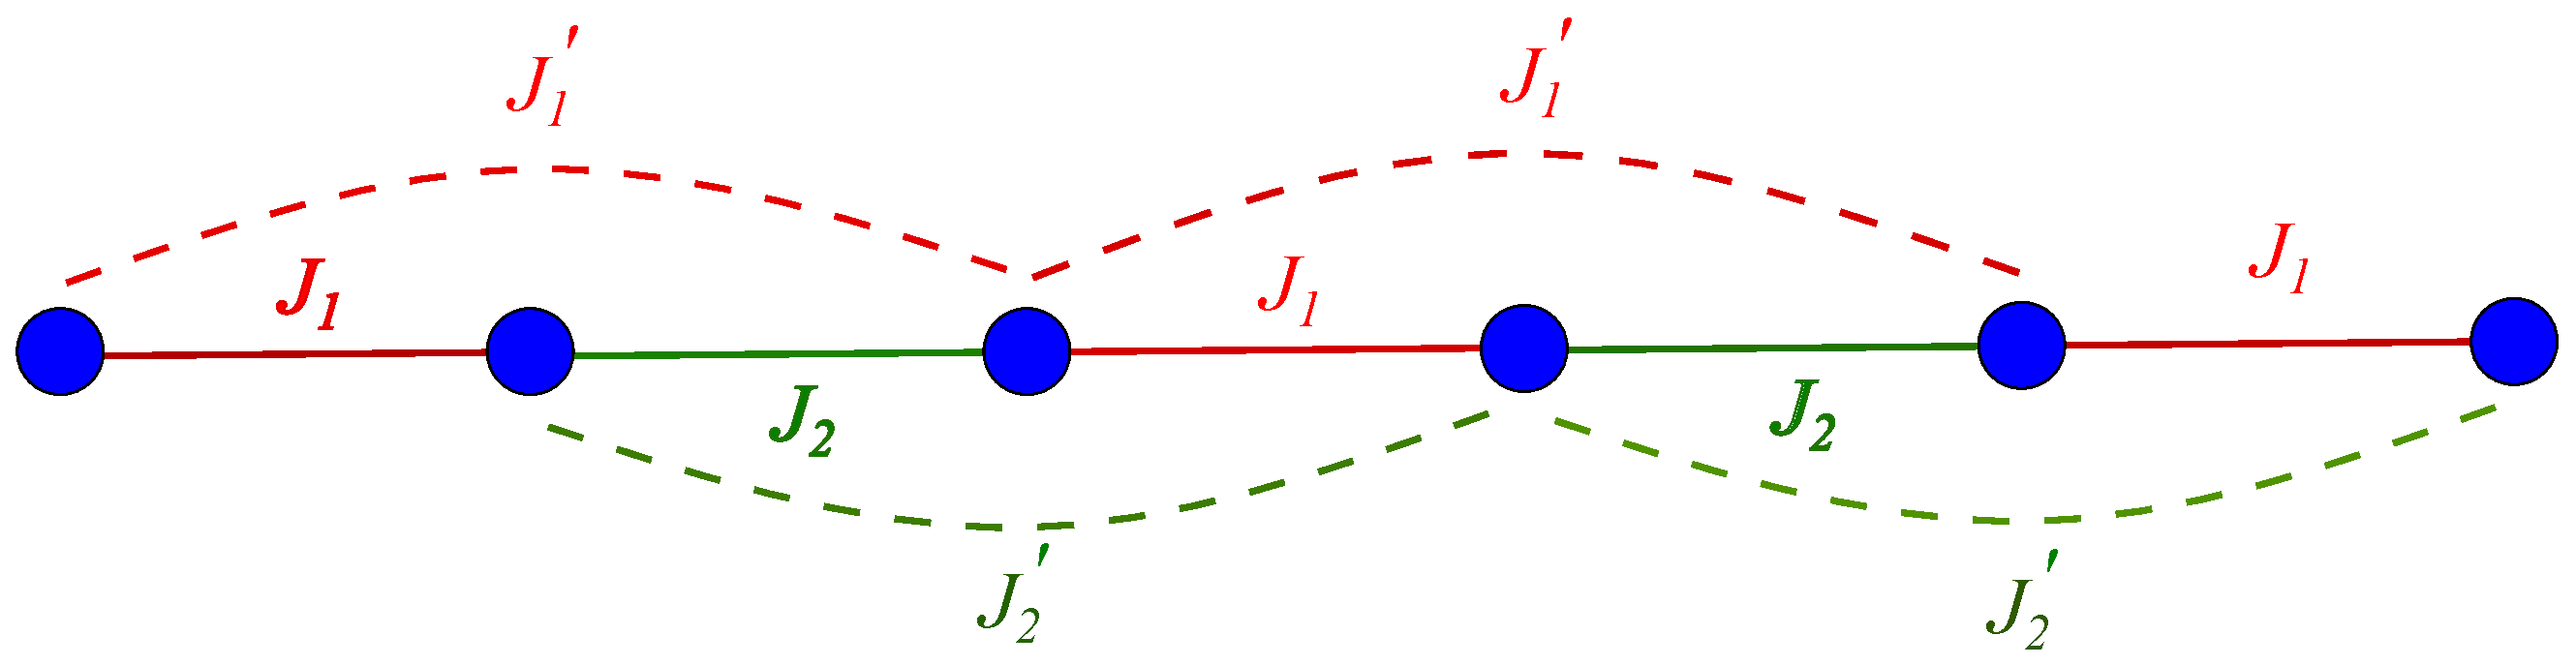
\includegraphics[width=0.8\linewidth]{part2/genChain.eps}}
 	\caption{Обобщенная модель Изинга с различными обменными взаимодействиями между ближайшими ($J_1, J_2$) и вторыми ($J_1^{'}, J_2^{'}$) соседями с трансляцией на два периода цепочки}
 	\label{genChain}
 \end{figure}

На рисунке~\ref{genChain} проиллюстрирована цепочка, соответствующая обобщенной модели Изинга, описываемой гамильтонианом \eqref{9}.

Определяем секулярное уравнение трансфер-матрицы $W_2$ в форме
\begin{equation}
\det (W_2-\lambda E) = 0,
\label{12}
\end{equation}
переписав его в виде
\begin{equation}
\lambda^4 + a\lambda^3 +b\lambda^2 + c\lambda + d = 0,
\label{13}
\end{equation}
решаем его~\cite{korn1970} и находим наибольшее собственное значение, которое принимает вид
\begin{multline}
\lambda_{\text{max}}=\frac{\sqrt{a^2-4b+4y}-a}{4}+\\+\sqrt{\left(\frac{\sqrt{a^2-4b+4y}-a}{4}\right)^2-\frac{y}{2}-\frac{2c-ya}{2\sqrt{a^2-4b+4y}}},
\label{14}
\end{multline}
где
\begin{align*}
Q&=\frac{p^3}{27}+\frac{q^2}{4};\;\;\;\; p=-\frac{b^2}{3}+ac-4d,\\
q&=-\frac{2b^3}{27}+\frac{bac}{3}+\frac{8bd}{3}-a^2d-c^2;\;\;\;	y=\sqrt[3]{\sqrt{Q}-\frac{q}{2}}+\sqrt[3]{-\sqrt{Q}-\frac{q}{2}}+\frac{b}{3}, \\
a&=-2\exp{\bigg(\frac{J_{1}^{'}+J_{2}^{'}}{T}\bigg)}\left(\ch \left( \frac{2H}{T}\right)\exp{\bigg(\frac{J_{1}+J_{2}}{T}\bigg)}+\exp{\bigg(\frac{-J_{1}-J_{2}}{T}\bigg)}\right), \\
b&= 4\exp{\bigg(\frac{2J_1^{'}+2J_2^{'}}{T}\bigg)}\ch \left( \frac{2H}{T}\right)-4\ch \bigg(\frac{2J_1^{'}-2J_2^{'}}{T}\bigg)\ch \left( \frac{2H}{T}\right) +\\&+ 2\exp{\bigg(\frac{-2J_1}{T}\bigg)} \sh \bigg(\frac{2J_1^{'}+2J_{2}^{'}-2J_{2}}{T}\bigg)
+\\&+ 2\exp{\bigg(\frac{2J_1}{T}\bigg)} \sh \bigg(\frac{2J_{1}^{'}+2J_{2}^{'}+2J_{2}}{T}\bigg),\\
c&=-8\exp{\bigg(\frac{J_{1}^{'}+J_{2}^{'}}{T}\bigg)}\left(\exp{\bigg(\frac{J_{1}+J_{2}}{T}\bigg)} +\right.\\&\left.+ \exp{\bigg(\frac{-J_{1}-J_{2}}{T}\bigg)} \ch \left(\frac {2H}{T} \right)\right) \sh \bigg(\frac{2J_{1}^{'}}{T}\bigg) \sh \bigg(\frac{2J_{2}^{'}}{T}\bigg),\\
d&=16\sh^2 \left(\frac{2J_{1}^{'}}{T}\right)\sh^2 \left(\frac {2J_{2}^{'}}{T}\right).
\end{align*}

Поскольку рассматривается перенос только на два периода трансляции цепочки ($n = 2$), то для нахождения термодинамических и магнитных величин системы необходимо воспользоваться формулами
\begin{equation}
F(H,T)=-\frac{T \ln \lambda_{\text{max}}}{2},
\end{equation}
\begin{equation}
S(H,T)=\frac{\ln \lambda_{\text{max}}}{2}+\frac{T}{2\lambda_{\text{max}}}\frac{\partial \lambda_{\text{max}}}{\partial T},
\end{equation}
\begin{equation}
C(H,T)=\frac{T}{2\lambda_{\text{max}}}\frac{\partial \lambda_{\text{max}}}{\partial T} + \frac{T}{2}\frac{\partial }{\partial T}\bigg(\frac{T}{\lambda_{\text{max}}}\frac{\partial \lambda_{\text{max}}}{\partial T}\bigg),
\end{equation}
\begin{equation}
M(H,T)=\frac{T}{2\lambda_{\text{max}}}\frac{\partial \lambda_{\text{max}}}{\partial H},
\end{equation}
\begin{equation}
E(H,T)=\frac{T^2}{2}\frac{\partial \lambda_{\text{max}}}{\partial T}.
\end{equation}


\section{Термодинамические, магнитные и фрустрационные свойства обобщенной модели Изинга}\label{sec:ch2/vector}

Детальный анализ большого количества всевозможных вариантов величин и знаков обменных взаимодействий показал, что при учете только двух различных обменов как между ближайшими, так и вторыми соседями в магнитном поле, система обладает семью магнитными конфигурациями в основном состоянии (в отличие от шести конфигураций в основном состоянии в случае отсутствия магнитного поля, см. статью~[A2]): антиферромагнитная структура 
\begin{equation*}
C_2 =
\left\{\!\begin{aligned}
&\dots \downarrow\;\;\; \uparrow \;\;\;\downarrow \;\;\; \uparrow   \dots\\[1ex]
& \dots \uparrow\;\;\; \downarrow \;\;\;\uparrow \;\;\; \downarrow  \dots
\end{aligned}\right\}
\end{equation*}
с внутренней энергией $E_{C_2} = (J_1+J_2)/2-(J_{1}^{'}+J_{2}^{'})/2$, ферромагнитное упорядочение 
\begin{equation*}
C_1 =
\left\{\!\begin{aligned}
\dots \uparrow\;\;\; \uparrow \;\;\;\uparrow \;\;\; \uparrow  \dots
\end{aligned}\right\}
\end{equation*}
с внутренней энергией	$E_{C_1} = -(J_1+J_2)/2-(J_{1}^{'}+J_{2}^{'})/2-H$, четыре фазы $C_{4}$, $C_{4}^{'}$, $C_{4}^{''}$ и $C_{4}^{'''}$ с учетверением периода трансляции решетки 
\begin{equation*}
C_4 =
\left\{\!\begin{aligned}
\dots \downarrow\;\;\; \downarrow \;\;\;\uparrow \;\;\; \uparrow  \dots \\[1ex]
\dots \uparrow\;\;\; \uparrow \;\;\;\downarrow \;\;\; \downarrow  \dots  
\end{aligned}\right\}
\;\;\;\;\;\;\;\;
C_4^{'} =
\left\{\!\begin{aligned}
\dots \uparrow\;\;\; \downarrow \;\;\;\downarrow \;\;\; \uparrow \dots \\[1ex] 
\dots \downarrow\;\;\; \uparrow \;\;\;\uparrow \;\;\; \downarrow \dots 
\end{aligned}\right\}
\end{equation*}
\begin{equation*}
C_4^{''} =
\left\{\!\begin{aligned}
\dots  \uparrow\;\;\; \uparrow \;\;\;\downarrow \;\;\; \uparrow  \dots  
\end{aligned}\right\}
\;\;\;\;\;\;\;\;
C_4^{'''} =
\left\{\!\begin{aligned}
\dots \uparrow\;\;\; \uparrow \;\;\;\uparrow \;\;\; \downarrow \dots 
\end{aligned}\right\}
\end{equation*}
с внутренними энергиями $E_{C_4} = -(J_1-J_2)/2+(J_{1}^{'}+J_{2}^{'})/2$, $E_{C_4^{'}} = (J_1--J_2)/2+(J_{1}^{'}+J_{2}^{'})/2$, $E_{C_4^{''}} = (J_{1}^{'}-J_{2}^{'})/2-H/2$, $E_{C_4^{'''}} = -(J_{1}^{'}-J_{2}^{'})/2-H/2$ соответственно и конфигурация $C_3$ с утроением периода трансляции
\begin{equation*}
C_3 =
\left\{\!\begin{aligned}
\dots \uparrow\;\;\; \uparrow \;\;\;\downarrow   \dots 
\end{aligned}\right\}
\end{equation*}
с внутренней энергией $E_{C_3} = (J_1+J_2+J_{1}^{'}+J_{2}^{'})/6-H/3$.

Рассматриваемая обобщенная модель Изинга в магнитном поле обладает восемью вариантами конкурирующих взаимодействий между ближайшими и вторыми соседями. Обсудим каждый из них отдельно. Но для начала введем коэффициенты взаимодействий: $R_1 = |J_1^{'} /J_1|$ и $R_2 = |J_2^{'} /J_2|$. Коэффициент $R_1$ отвечает за отношение взаимодействий на нечетных узлах решетки, а $R_2$ на четных узлах.		

 \begin{figure}[h]
 	\center{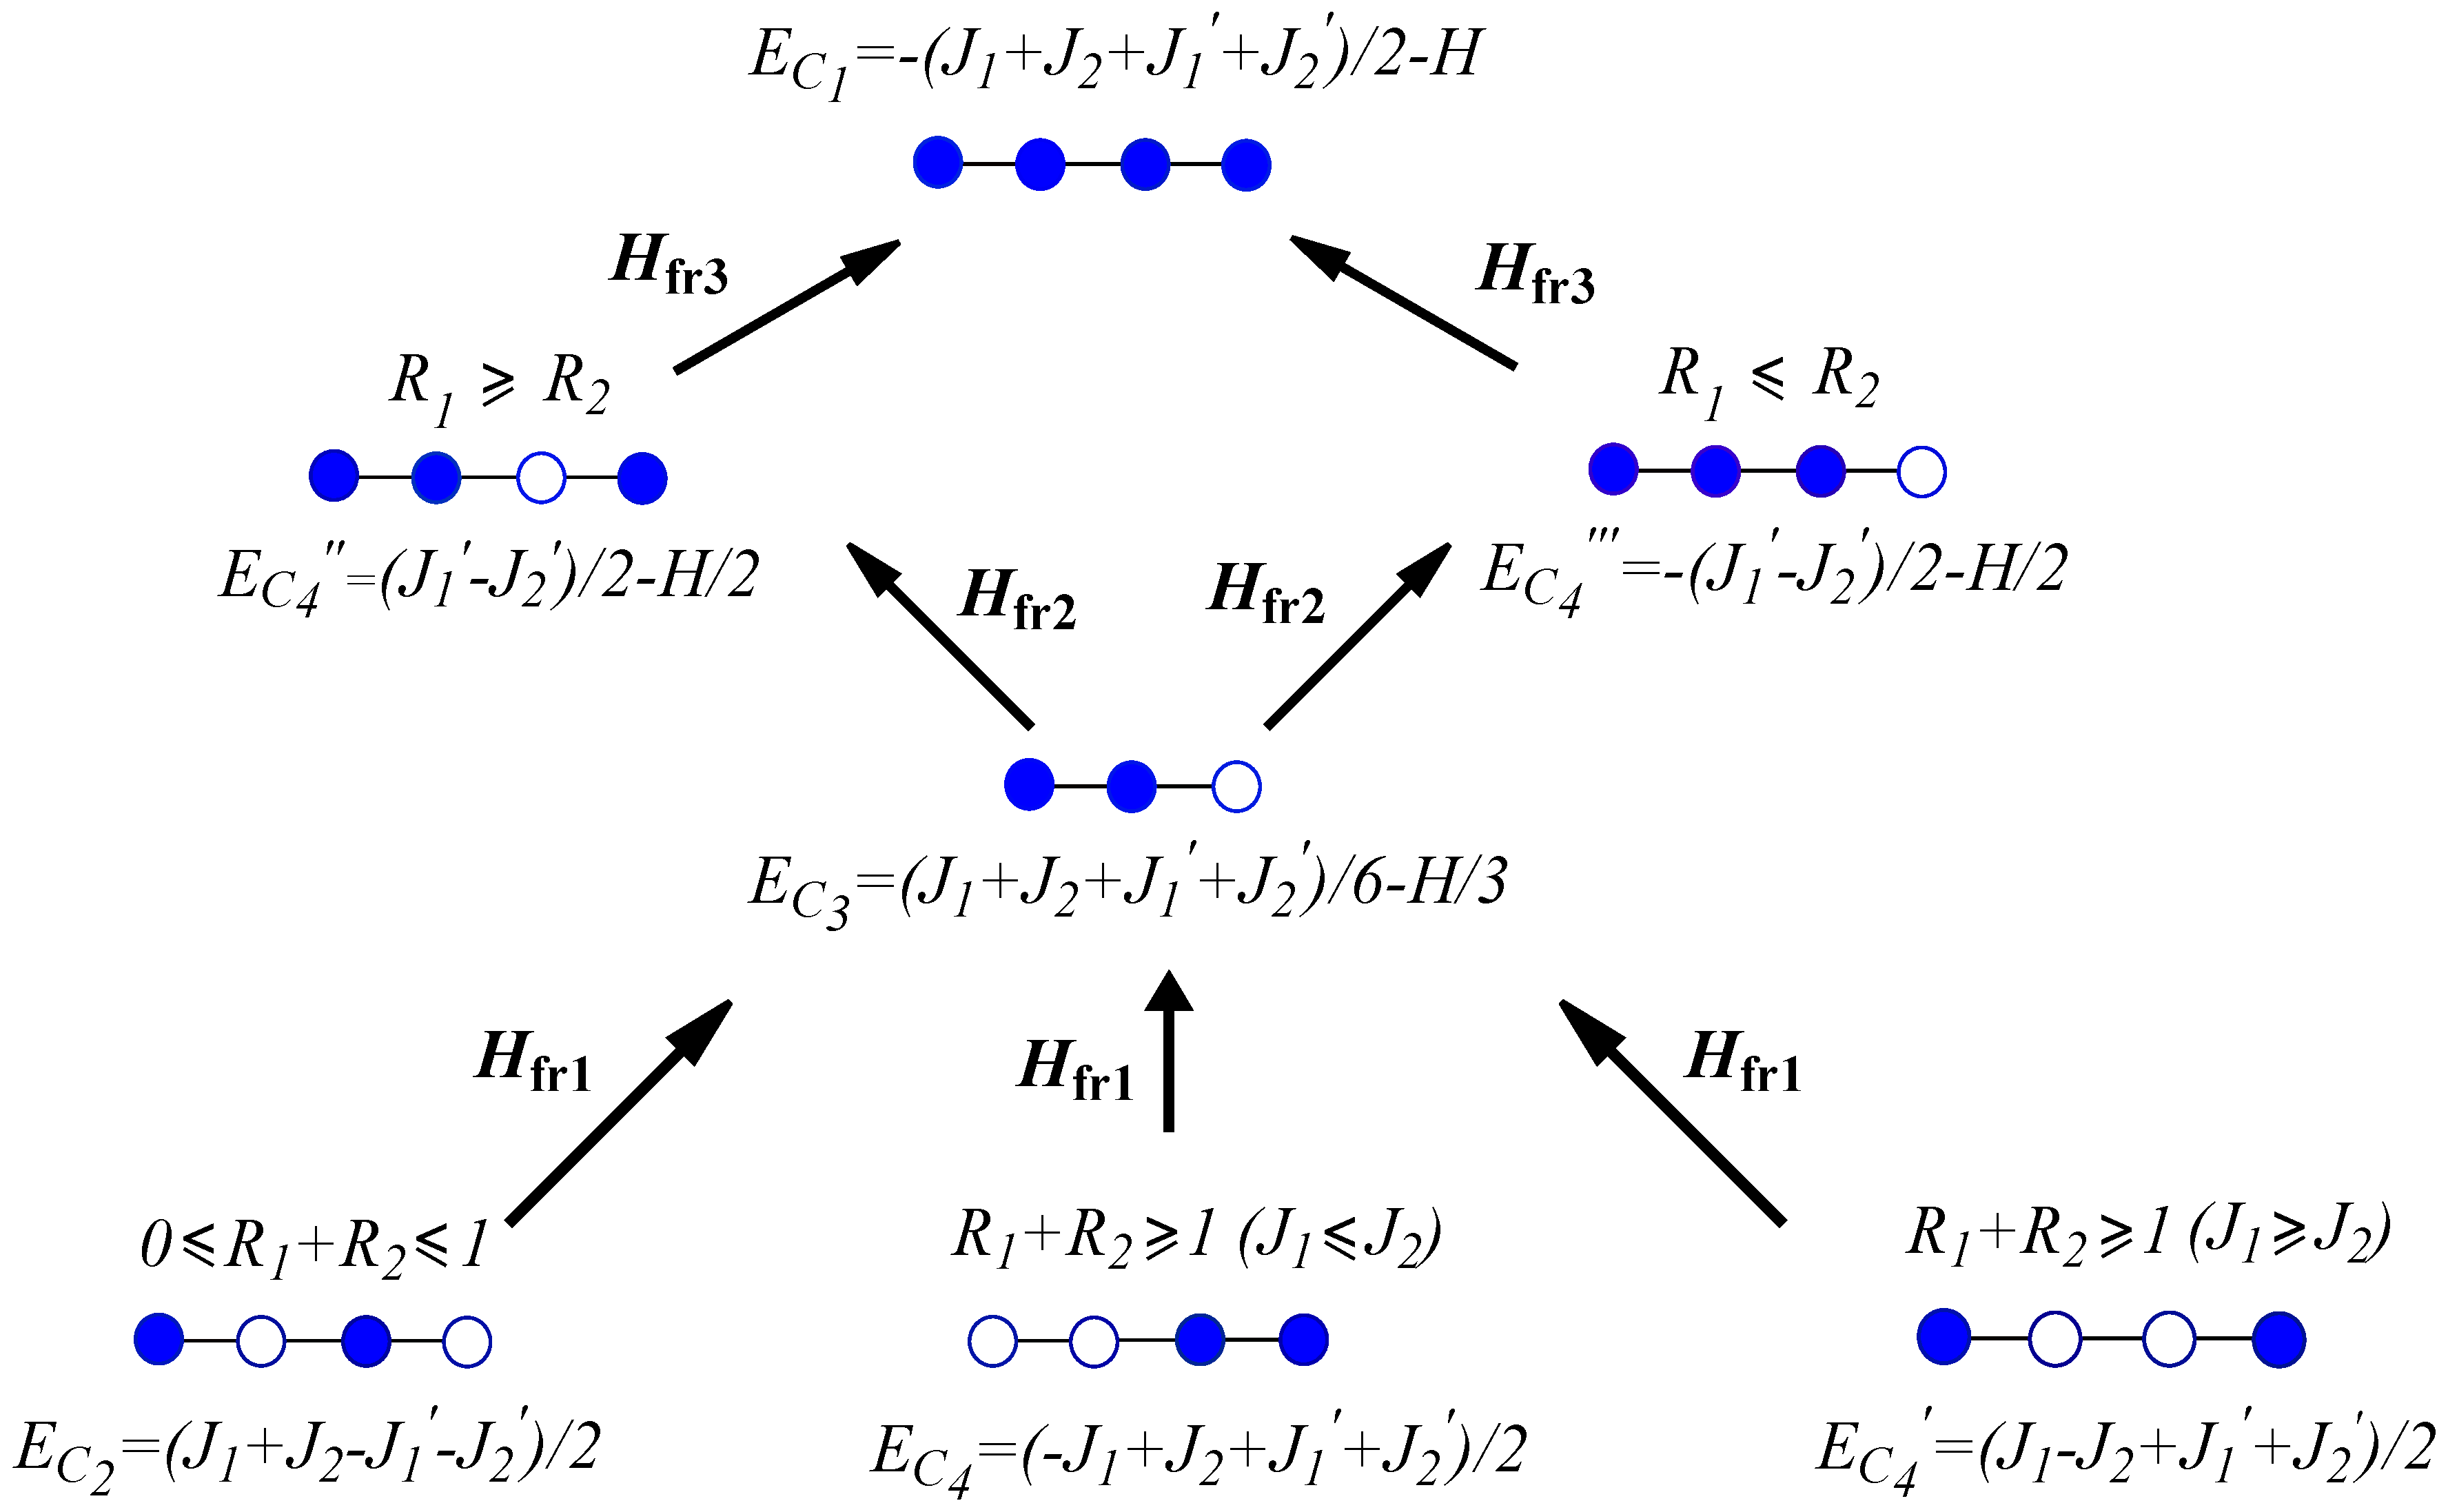
\includegraphics[width=0.8\linewidth]{part2/transGenChain1.eps}}
 	\caption{Схема переходов в варианте конкурирующих взаимодействий при $J_1 < 0$, $J_1^{'} < 0$, $J_2 < 0$, $J_2^{'} < 0$. Сплошные кружочки --- спин направлен вверх, пустые --- вниз}
 	\label{transGenChain1}
 \end{figure}

1.~\emph{Антиферромагнитные взаимодействия между ближайшими и вторыми соседями ($J_1 < 0, J_1^{'} < 0, J_2 < 0, J_2^{'} < 0$)}

Сравнивая энергии конфигураций (рис.~\ref{transGenChain1}), установленных выше, определим фрустрационные поля, в которых происходят переходы между соответствующими упорядочениями
\[
\begin{aligned}
H_{\text{fr$_1$}}&=
\begin{cases}
-J_1+2J_1^{'}-J_2+2J_2^{'}, & \text{ при }  0\leq R_1+R_2\leq 1; \\
2J_1-J_1^{'}-J_2-J_2^{'},   & \text{ при }  R_1+R_2\ge 1 \text{ и } J_{1}\leq J_{2}; \\
-J_1-J_1^{'}+2J_2-J_2^{'}, & \text{ при }  R_1+R_2\ge 1 \text{ и } J_{1}\ge J_{2}.
\end{cases}\\
\end{aligned}
\]

\[
\begin{aligned}
H_{\text{fr$_2$}}&=
\begin{cases}
-J_1+2J_1^{'}-J_2-4J_2^{'}, & \text{ при }  R_1\ge R_2; \\
-J_1-4J_1^{'}-J_2+2J_2^{'},   & \text{ при }  R_1\leq R_2.
\end{cases}\\
\end{aligned}
\]

\[
\begin{aligned}
H_{\text{fr$_3$}}&=
\begin{cases}
-J_1-2J_1^{'}-J_2, & \text{ при }  R_1\ge R_2; \\
-J_1-J_2-2J_2^{'},   & \text{ при }  R_1 \leq R_2.
\end{cases}\\
\end{aligned}
\]

\emph{Первое фрустрирующее поле при $R_1 + R_2 < 1$}. Данное фрустрирующее поле получается при рассмотрении перехода между антиферромагнитной конфигурацией $C_2$ и конфигурацией $C_3$ с утроением периода трансляций решетки~\cite{zarubin2019}. Значение нуль-температурной энтропии находится как натуральный логарифм единственного вещественного корня уравнения \mbox{$x^3-x-1=0$}, известного как пластическое число
\begin{equation}
S_{T\rightarrow 0} = \ln \rho = 0.2812\dots,
\label{15}
\end{equation}
где $\rho = \sqrt[3]{(9+\sqrt{69})/18}+\sqrt[3]{(9-\sqrt{69})/18}$ --- пластическое число.

Значение нуль-температурной намагниченности, в свою очередь, может быть выражено через пластическое число
\begin{equation}
M_{T\rightarrow 0} = \frac{1}{3\rho^3-\rho} = 0.1770\dots
\label{16}
\end{equation}


\emph{Первое фрустрирующее поле при $R_1 + R_2 > 1$ и $J_1 < J_2$ или при $R_1 + R_2 > 1$ и $J_1 > J_2$}. В этом фрустрирующем поле возникает переход между фазами учетверения периода трансляций решетки и между фазой утроения периода трансляций, а именно, между фазами $C_4$ и $C_3$ либо между
фазами $C_4^{'}$ и $C_3$, в зависимости от величин $J_1$ и $J_2$. Значение энтропии при стремлении температуры к нулю равно натуральному логарифму квадратного корня из пластического числа
\begin{equation}
S_{T\rightarrow 0} = \ln \sqrt{\rho} = 0.1406\dots
\label{17}
\end{equation}
Соответствующая намагниченность равна выражению \eqref{16}.

\emph{Первое фрустрирующее поле при $R_1 + R_2 > 1$ и $J_1 = J_2$}. В случае, когда $J_1 = J_2$, энергии конфигураций с учетверением периода трансляций $C_4$ и $C_4^{'}$ станут равны, тем самым, фрустрирующие поля также совпадут~\cite{zarubin2019}. Нуль-температурная энтропия находится как натуральный логарифм наибольшего вещественного корня уравнения $x^4-x-1=0$
\begin{equation}
S_{T\rightarrow 0} = \ln \xi = 0.1995\dots,
\label{18}
\end{equation}
а нуль-температурная намагниченность
\begin{equation}
M_{T\rightarrow 0} = \frac{1}{\xi+4\xi^3-\xi^4} = 0.1593\dots,
\label{19}
\end{equation}
при 
\begin{equation*}
\xi = \sqrt{\alpha- \beta} + \sqrt{\frac{1}{4\sqrt{\alpha - \beta}}-\alpha+\beta},
\end{equation*}
где $\alpha = \sqrt[3]{(\sqrt{849}+9)/1152}$, $\beta = \sqrt[3]{(\sqrt{849}-9)/1152}$.
Полученное математическое сечение пока безымянное.

\emph{Первое фрустрирующее поле при $R_1 + R_2 = 1$}. При таком условии система вырождается в обычную (не обобщенную)
модель Изинга с взаимодействиями между ближайшими и вторыми соседями~\cite{zarubin2019}. Фрустрирующее поле равно нулю, а энтропия равна натуральному логарифму золотого сечения 
\begin{equation}
S_{T\rightarrow 0} = \ln \varphi = 0.4812\dots
\label{20}
\end{equation}

Стоит отметить, что теория магнетизма, построенная в обычной модели Изинга с учетом взаимодействий между ближайшими и вторыми соседями, была применена несколькими учеными для объяснения поведения соединений CoCl$_2$ ·$2$H$_2$0 и CoBr$_2$ · $2$H$_2$0 в магнитном поле~\cite{oguchi1965, narath1964, kobayashi1964}.

\emph{Второе фрустрирующее поле при $R_1 > R_2$ или $R_1 < R_2$}. Если $R_1 > R_2$, то система претерпевает переход в конфигурацию учетверения $C_4^{''}$ из фазы утроения периода трансляций $C_3$, а если $R_1 < R_2$, тогда система перейдет в конфигурацию $C_{4}^{'''}$ из фазы $C_3$.
Тем не менее, значения нуль-температурных энтропий для этих двух переходов будут одинаковы \eqref{17}, как и намагниченности
\begin{equation}
M_{T\rightarrow 0} = \frac{\rho^2}{3\rho^2-1} = 0.4115\dots,
\label{21}
\end{equation}
где $\rho = \sqrt[3]{(9+\sqrt{69})/18}+\sqrt[3]{(9-\sqrt{69})/18}$ --- пластическое число.

\emph{Второе фрустрирующее поле при $R_1 = R_2$}. При равенстве коэффициентов взаимодействий $R_1$ и $R_2$ получаем обычную (не обобщенную) модель Изинга с взаимодействиями между первыми и вторыми соседями в магнитном поле. Происходит переход из конфигурации с утроением периода трансляций $C_3$ сразу в ферромагнитную конфигурацию $C_1$~\cite{zarubin2019}. Нуль-температурная энтропия в данном фрустрирующем поле выражается как натуральный логарифм единственного вещественного корня уравнения \mbox{$x^3-x^2-1=0$}, известного как сверхзолотое сечение
\begin{equation}
S_{T\rightarrow 0} = \ln \psi = 0.3822\dots,
\label{22}
\end{equation}
а нуль-температурная намагниченность равна
\begin{equation}
M_{T\rightarrow 0} = \frac{\psi^3}{\psi^2+3} = 0.6115\dots,
\label{23}
\end{equation}
где $\psi = \Big(1+\sqrt[3]{(29+3\sqrt{93})/2}+\sqrt[3]{(29-3\sqrt{93})/2}\Big)/3$ --- сверхзолотое сечение.

\emph{Третье фрустрирующее поле при $R_1 < R_2$ или $R_1 > R_2$}. В данном фрустрирующем поле происходит переход из конфигураций с учетверением  периода трансляций $C_{4}^{''}$ (или $C_4^{'''}$) в ферромагнитное состояние $C_1$. Значение нуль-температурной энтропии равно натуральному логарифму квадратного корня из золотого сечения
\begin{equation}
S_{T\rightarrow 0} = \ln \sqrt{\varphi} = 0.2406\dots
\label{24}
\end{equation}
а нуль-температурная намагниченность
\begin{equation}
M_{T\rightarrow 0} = \frac{\varphi}{2\varphi -1} = 0.7236\dots
\label{25}
\end{equation}

 \begin{figure}[h]
 	\begin{minipage}{0.47\linewidth}
 		\center{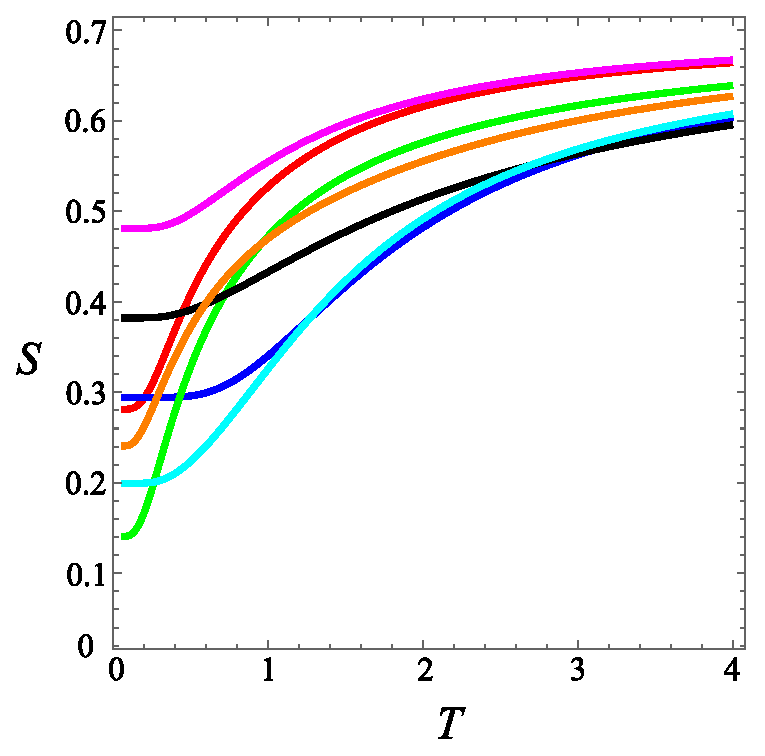
\includegraphics[width=1\linewidth]{part2/entropyGenChain1.eps} \\ а)}
 	\end{minipage}
 	\hfill
 	\begin{minipage}{0.47\linewidth}
 		\center{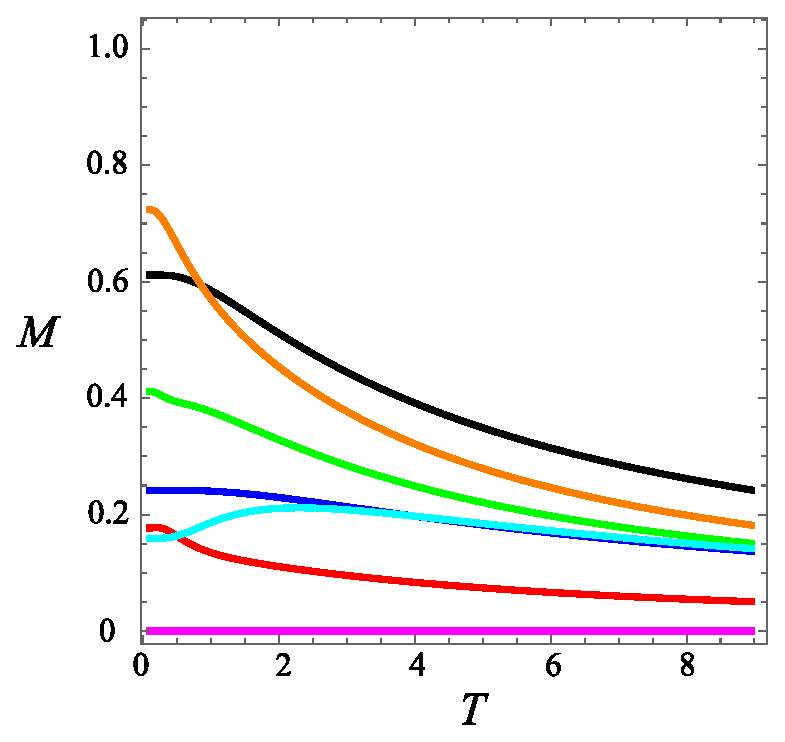
\includegraphics[width=1\linewidth]{part2/magGenChain1.eps} \\ б)}
 	\end{minipage}
 	\caption{Температурные зависимости а) энтропий, б) намагниченностей. Зеленые кривые --- $J_1 = -1$, $J_1^{'} = -0.5$, $J_2 = -1$, $J_2^{'} = -0.2$, $H = 1.8$, красные кривые --- $J_1 = -1$, $J_1^{'} = -0.5$, $J_2 = -1$, $J_2^{'} = -0.2$, $H = 0.6$, синие кривые --- $J_1 = -1$, $J_1^{'} = -2$, $J_2 = -1$, $J_2^{'} = -1$, $H = 2$, черные кривые --- $J_1 = -1$, $J_1^{'} = -0.5$, $J_2 = -1$, $J_2^{'} = -0.5$, $H = 3$, фиолетовые кривые --- $J_1 = -1$, $J_1^{'} = -0.5$, $J_2 = -1$, $J_2^{'} = -0.5$, $H = 0$, оранжевые кривые --- $J_1 = -0.2$, $J_1^{'} = -0.4$, $J_2 = -1$, $J_2^{'} = -0.2$, $H = 2$, бирюзовые кривые --- $J_1 = -1$, $J_1^{'} = -1.5$, $J_2 = -1$, $J_2^{'} = -1.6$, $H = 2.1$}
 	\label{EntAndMagGenChain1}
 \end{figure}


Однако, если положить $|R_1 - R_2| = 1$, первое и второе фрустрирующие поля совпадут ($H_{\text{fr}_1} = H_{\text{fr}_2}$), при этом произойдет переход из конфигураций с нулевой намагниченностью ($C_2$, $C_4$ или $C_4^{'}$) непосредственно в фазу с учетверением периода трансляций решетки ($C_4^{''}$ или $C_4^{'''}$), энтропия в этом случае находится как натуральный логарифм квадратного корня наибольшего решения уравнения $x^3-x^2-2x+1=0$
\begin{equation}
S_{T\rightarrow 0} = \ln \sqrt{\nu} = 0.2944\dots,
\label{26}
\end{equation}
\begin{equation}
M_{T\rightarrow 0} = \frac{1}{3\nu^2-2\nu-2} = 0.2417\dots,
\label{27}
\end{equation}
где $\nu = \Big(1+\sqrt[3]{98/(3\sqrt{3}i-1)}+\sqrt[3]{(21\sqrt{3}i-7)/2}\Big)/3$. Это математическое сечение пока безымянное.

Перечисленные фрустрационные значения энтропий и намагниченностей отражены на рисунке~\ref{EntAndMagGenChain1}.

 \begin{figure}[h]
 	\center{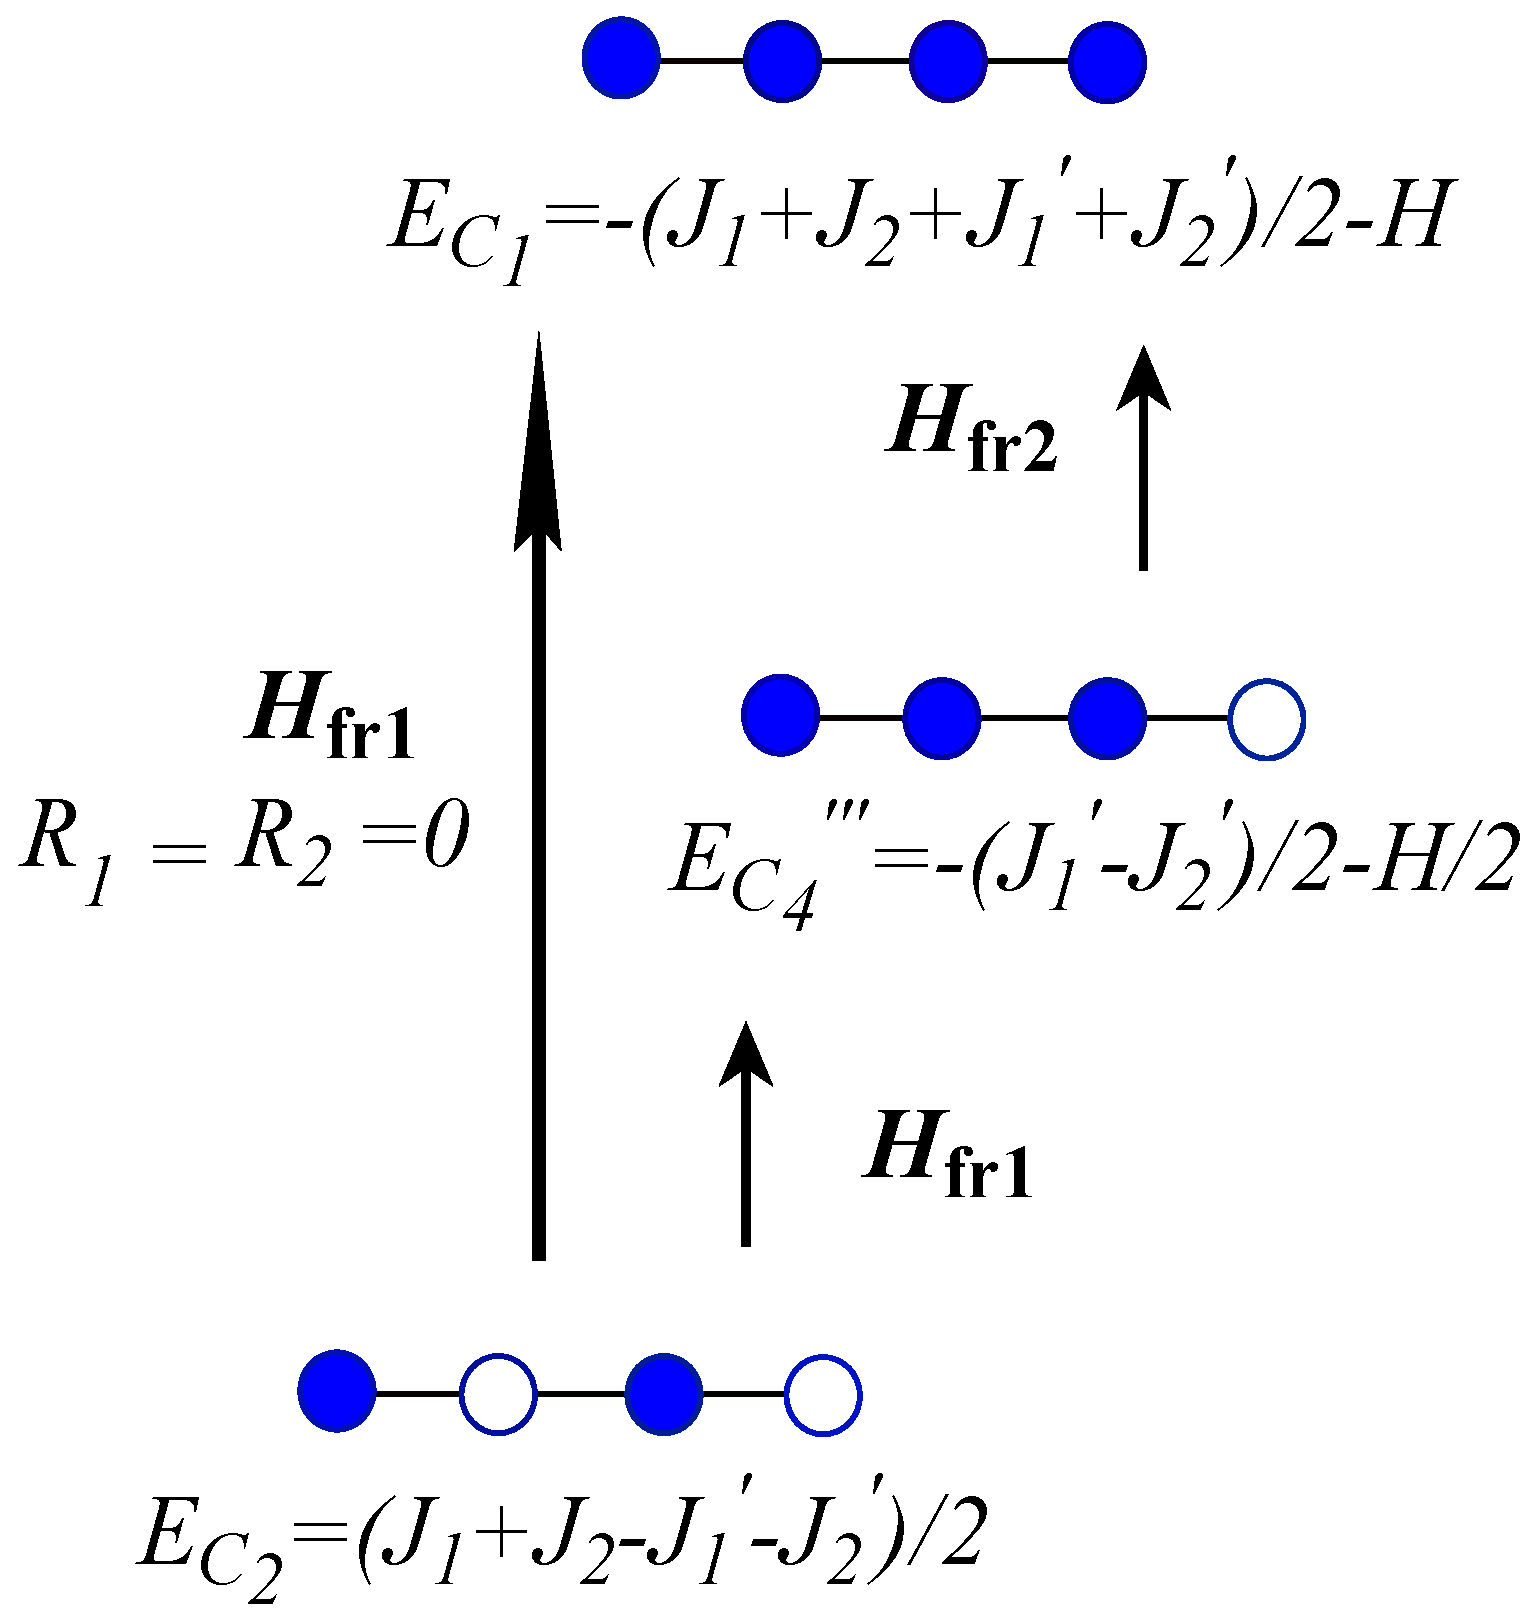
\includegraphics[width=0.4\linewidth]{part2/transGenChain2.eps}}
 	\caption{Вариант конкурирующих взаимодействий при $J_1 < 0$, $J_1^{'} > 0$, $J_2 < 0$, $J_2^{'} < 0$. Сплошные кружочки --- спин направлен вверх, пустые --- вниз}
 	\label{transGenChain2}
 \end{figure}

2.~\emph{Антиферро-антиферромагнитное взаимодействие между ближайшими соседями, антиферро-ферромагнитное взаимодействие между вторыми соседями ($J_1<0, J_{1}^{'}<0, J_{2}<0, J_{2}^{'}>0$)}

\[
\begin{aligned}
H_{\text{fr}_1}&=-J_1+2J_{1}^{'}-J_{2};\\
H_{\text{fr}_2}&= -J_1-2J_1^{'}-J_2.
\end{aligned}
\]

3.~\emph{Антиферро-антиферромагнитное взаимодействие между ближайшими соседями, ферро-антиферромагнитное взаимодействие между вторыми соседями ($J_1<0, J_{1}^{'}>0, J_{2}<0, J_{2}^{'}<0$)}

\[
\begin{aligned}
H_{\text{fr}_1}&=-J_1-J_{2}+2J_{2}^{'};\\
H_{\text{fr}_2}&= -J_1-J_2-2J_2^{'}.
\end{aligned}
\]

Варианты этих двух конкурирующих взаимодействий схожи. Достаточно привести только одну схему переходов, например, $J_1 < 0$, $J_1^{'} > 0$, $J_2 < 0$, $J_2^{'} < 0$ (рис.~\ref{transGenChain2}). Отличительной чертой этих двух вариантов является только разница в промежуточном состоянии ($C_4^{''}$ или $C_4^{'''}$) между антиферромагнитной ($C_2$) и ферромагнитной ($C_1$) конфигурациями.

\emph{Первое фрустрирующее поле}. В данном фрустрирующем поле происходит переход из антиферромагнитного упорядочения $C_2$ в конфигурацию с учетверением периода трансляции $C_4^{'''}$. Энтропия равна натуральному логарифму корня из золотого сечения \eqref{24} с соответствующим значением намагниченности
\begin{equation}
M_{T\rightarrow 0} = \frac{1}{2\varphi^2 - \varphi} = 0.2763\dots
\label{28}
\end{equation}

\emph{Второе фрустрирующее поле}. Энтропия соответствует выражению \eqref{24}, а намагниченность
\begin{equation}
M_{T\rightarrow 0} = \frac{1}{2\varphi -1} = 0.4472\dots
\label{29}
\end{equation}

При $R_1 = R_2 = 0$ приходим к случаю не обобщенной модели Изинга с взаимодействием ближайших соседей в магнитном поле~\cite{zarubin2019} с хорошо известными значениями для нуль-температурных энтропий \eqref{20} и намагниченностей \eqref{29}.

4.~\emph{Антиферро-ферромагнитное взаимодействие между ближайшими соседями, ферро-антиферромагнитное взаимодействие между вторыми соседями ($J_1<0, J_{1}^{'}>0, J_{2}>0, J_{2}^{'}<0$)}

\[
\begin{aligned}
H_{\text{fr}_1}&=
\begin{cases}
-J_1-J_1^{'}-J_{2}^{'}, & \text{ при } 0\leq R_1+R_2\leq 1 ; \\
-J_1-2J_1^{'}+J_2,   & \text{ при } R_1+R_2\ge 1 .
\end{cases}\\
H_{\text{fr}_2}&= -J_1-J_2-2J_2^{'}.
\end{aligned}
\]
При $R_1\ge (|J_1|+|J_2|)/2, (|J_1|\ge 1, |J_2|\ge 1)$ и любом $R_2$: основное состояние $C_4^{'''}$.

5.~\emph{Антиферро-ферромагнитное взаимодействие между ближайшими и вторыми соседями ($J_1<0, J_{1}^{'}<0, J_{2}>0, J_{2}^{'}>0$)}

\[
\begin{aligned}
H_{\text{fr}_1}&=
\begin{cases}
-J_1-J_1^{'}-J_{2}^{'}, & \text{ при } 0\leq R_1+R_2\leq 1 ; \\
-J_1-2J_1^{'}+J_2,   & \text{ при } R_1+R_2\ge 1 .
\end{cases}\\
H_{\text{fr}_2}&= -J_1-2J_1^{'}-J_2.
\end{aligned}
\]
При $R_2\ge (|J_1|+|J_2|)/2, (|J_1|\ge 1, |J_2|\ge 1)$ и любом $R_1$: основное состояние $C_4^{''}$.

6.~\emph{Ферро-антиферромагнитное взаимодействие между ближайшими и вторыми соседями ($J_1>0, J_{1}^{'}>0, J_{2}<0, J_{2}^{'}<0$)}

\[
\begin{aligned}
H_{\text{fr}_1}&=
\begin{cases}
-J_1^{'}-J_2-J_2^{'}, & \text{ при } 0\leq R_1+R_2\leq 1 ; \\
J_1-2J_1^{'}-J_2,   & \text{ при }  R_1+R_2\ge 1.
\end{cases}\\
H_{\text{fr}_2}&= -J_1-J_2-2J_2^{'}.
\end{aligned}
\]
При $R_1\ge (|J_1|+|J_2|)/2, (|J_1|\ge 1, |J_2|\ge 1)$ и любом $R_2$: основное состояние $C_4^{'''}$.

7.~\emph{Ферро-антиферромагнитное взаимодействие между ближайшими соседями, антиферро-ферромагнитное взаимодействие между вторыми соседями ($J_1>0, J_{1}^{'}<0, J_{2}<0, J_{2}^{'}>0$) }

\[
\begin{aligned}
H_{\text{fr}_1}&=
\begin{cases}
-J_1^{'}-J_2-J_2^{'}, & \text{ при } 0\leq R_1+R_2\leq 1 ; \\
J_1-J_2-2J_2^{'},   & \text{ при }  R_1+R_2\ge 1.
\end{cases}\\
H_{\text{fr}_2}&= -J_1-2J_1^{'}-J_2.
\end{aligned}
\]
При $R_2\ge (|J_1|+|J_2|)/2, (|J_1|\ge 1, |J_2|\ge 1)$ и любом $R_1$: основное состояние $C_4^{''}$.

 \begin{figure}[h]
 	\center{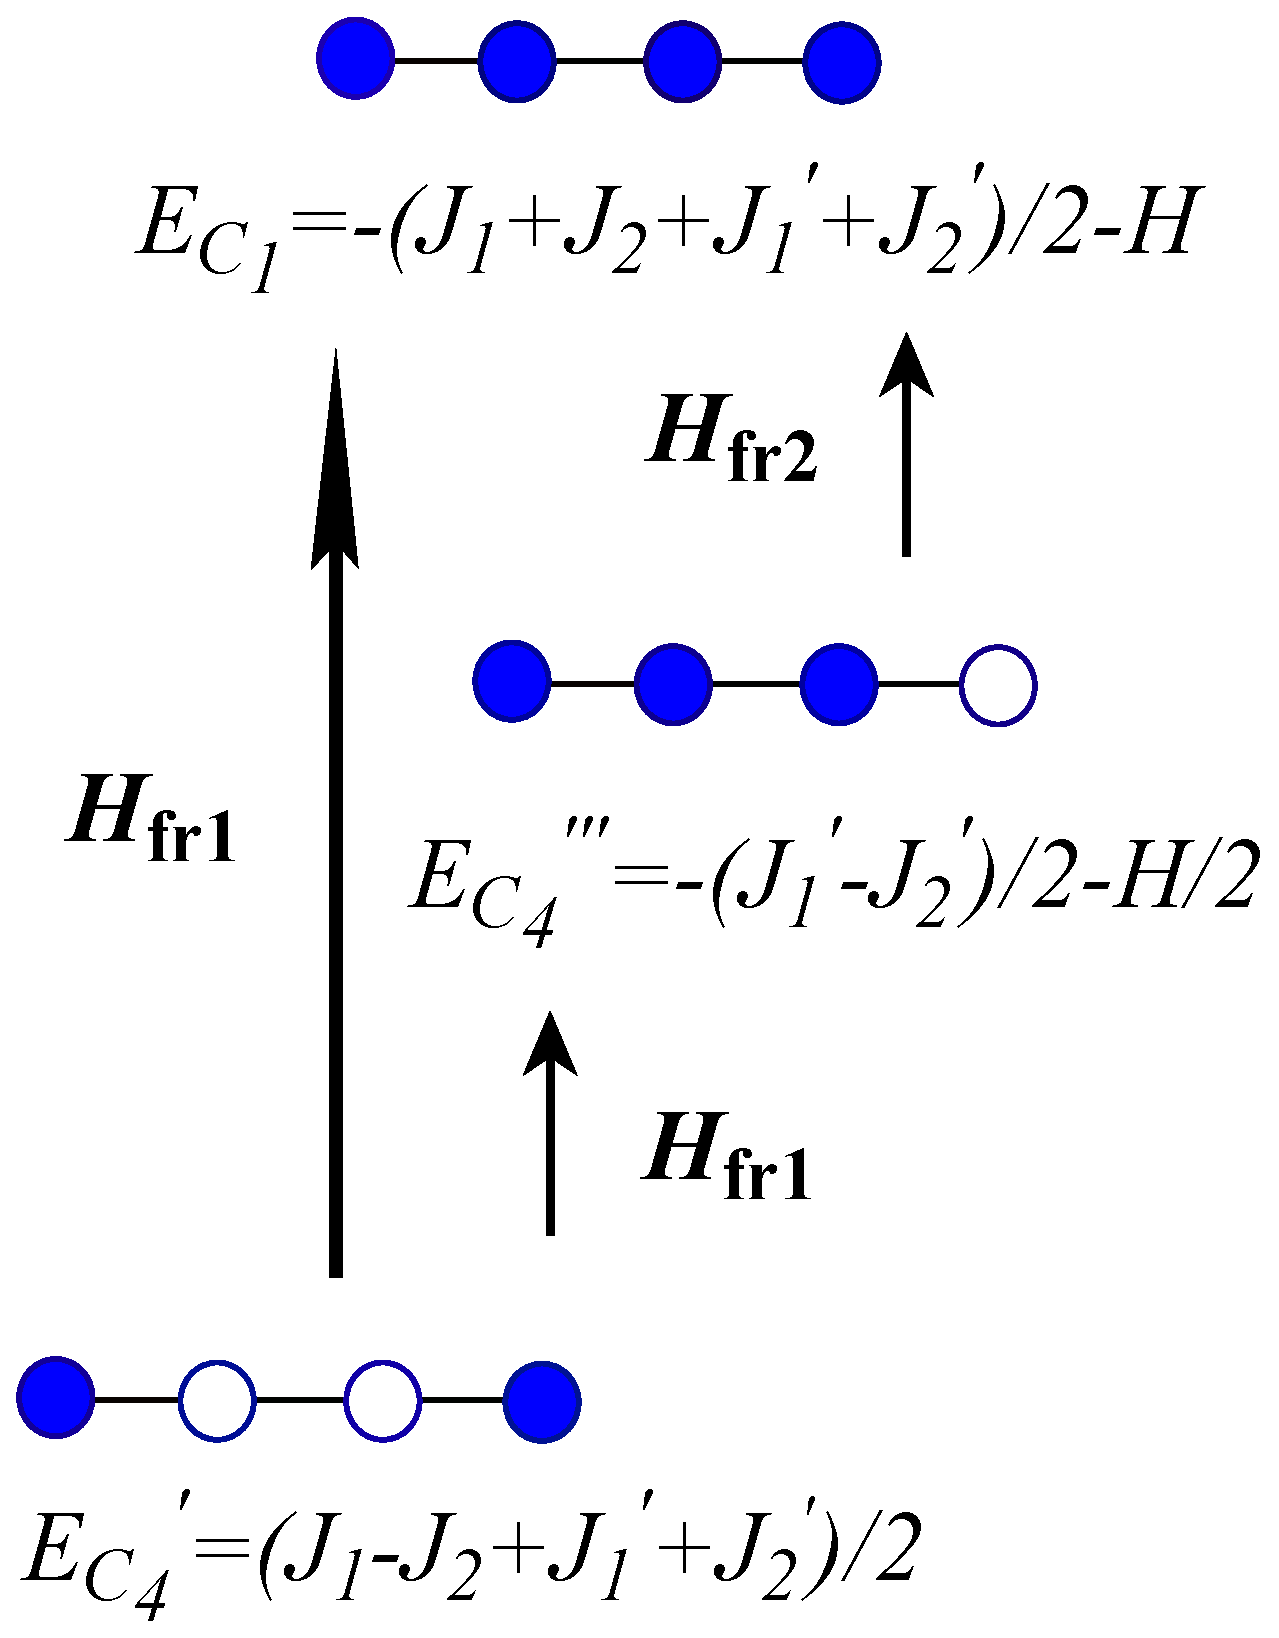
\includegraphics[width=0.35\linewidth]{part2/transGenChain3.eps}}
 	\caption{Возможные варианты переходов между конфигурациями в магнитном поле при $J_1 < 0$, $J_1^{'} > 0$, $J_2 > 0$, $J_2^{'} < 0$. Сплошные кружочки --- спин направлен вверх, пустые --- вниз}
 	\label{transGenChain3}
 \end{figure}

Характерной чертой четырех рассматриваемых вариантов является то, что один из коэффициентов взаимодействия может быть сколь угодно большим по модулю. Главное, чтобы знак этого взаимодействия сохранялся. Кроме того, если второй коэффициент достигает величины $(|J_1| + |J_2|)/2$ при $(|J_1| \ge 1, |J_2| \ge 1)$, то фаза с учетверением периода трансляций ($C_4^{''}$ или
$C_4^{'''}$) становится начальным состоянием системы.  На рисунке \ref{transGenChain3} приведена схема переходов при $J_1 < 0, J_1^{'} > 0, J_2 > 0, J_2^{'} < 0$.

\emph{Первое фрустрирующее поле при $0\leq R_1+R_2\leq 1$}. Энтропия находится из выражения \eqref{24}, а намагниченность из выражения \eqref{29}.

\emph{Первое фрустрирующее поле при $R_1 + R_2 \geqslant 1$}. Данное фрустрирующее поле описывает переход между фазами с учетверением периода трансляций, конкретнее, переход осуществляется из фазы $C_4^{''}$ в фазу $C_4^{'''}$. Нуль-температурная энтропия равна натуральному логарифму корня четвертой степени из двух
\begin{equation}
S_{T\rightarrow 0} = \ln \sqrt[4]{2} = 0.1733\dots,
\label{30}
\end{equation}
нуль-температурная намагниченность равна
\begin{equation}
M_{T\rightarrow 0} = \frac{1}{4}.
\label{31}
\end{equation}

\emph{Второе фрустрирующее поле}. Энтропия равна выражению \eqref{24}, намагниченность выражению \eqref{25}.

При $R_1 + R_2 = 1$ получается переход из фазы с учетверением периода трансляций $C_4^{'''}$ в ферромагнитную фазу $C_1$, при этом энтропия равна  натуральному логарифму квадратного корня из двух 
\begin{equation}
S_{T\rightarrow 0}=\ln \sqrt{2},
\label{32}
\end{equation}
а соответствующая намагниченность будет равна
\begin{equation}
M_{T\rightarrow 0} = \frac{1}{2}.
\label{33}
\end{equation}

Такое значение намагниченности символизирует то, что вдоль поля направлена половина всех спинов в цепочке.

8.~\emph{Ферромагнитное взаимодействие между ближайшими соседями, антиферромагнитное взаимодействие между вторыми соседями ($J_1>0$, $J_{1}^{'}<0$, $J_{2}>0$, $J_{2}^{'}<0$)}

Данный вариант является обобщением конкурирующих взаимодействий
между ближайшими соседями в обычной модели Изинга~\cite{zarubin2019}. Положим, что $J_1 = J_2$, таким образом, энергии конфигураций с учетверениями периода трансляций с нулевой намагниченностью совпадут. При увеличении магнитного поля будут происходить переходы в состояния с намагниченностью $1/2$, более того, при некоторых значениях обменных взаимодействий возможен переход сразу в ферромагнитную конфигурацию (рис.~\ref{transGenChain4}).

\[
\begin{aligned}
H_{\text{fr}_1}&=
\begin{cases}
J_{1}-J_2-2J_{2}^{'}, & \text{ при } R_1-R_2\ge 1; \\
-J_{1}^{'}-J_2-J_{2}^{'}, & \text{ при } -1\leq R_1-R_2\leq 1; \\
J_1-2J_{1}^{'}-J_{2},   & \text{ при }  R_1-R_2\leq  -1.
\end{cases}\\
H_{\text{fr}_2}&=
\begin{cases}
-J_1-2J_1^{'}-J_2, & \text{ при } R_1-R_2\ge 1; \\
-J_1-J_2-2J_2^{'},   & \text{ при }  R_1-R_2\leq -1.
\end{cases}\\
\end{aligned}
\]

 \begin{figure}[h]
 	\center{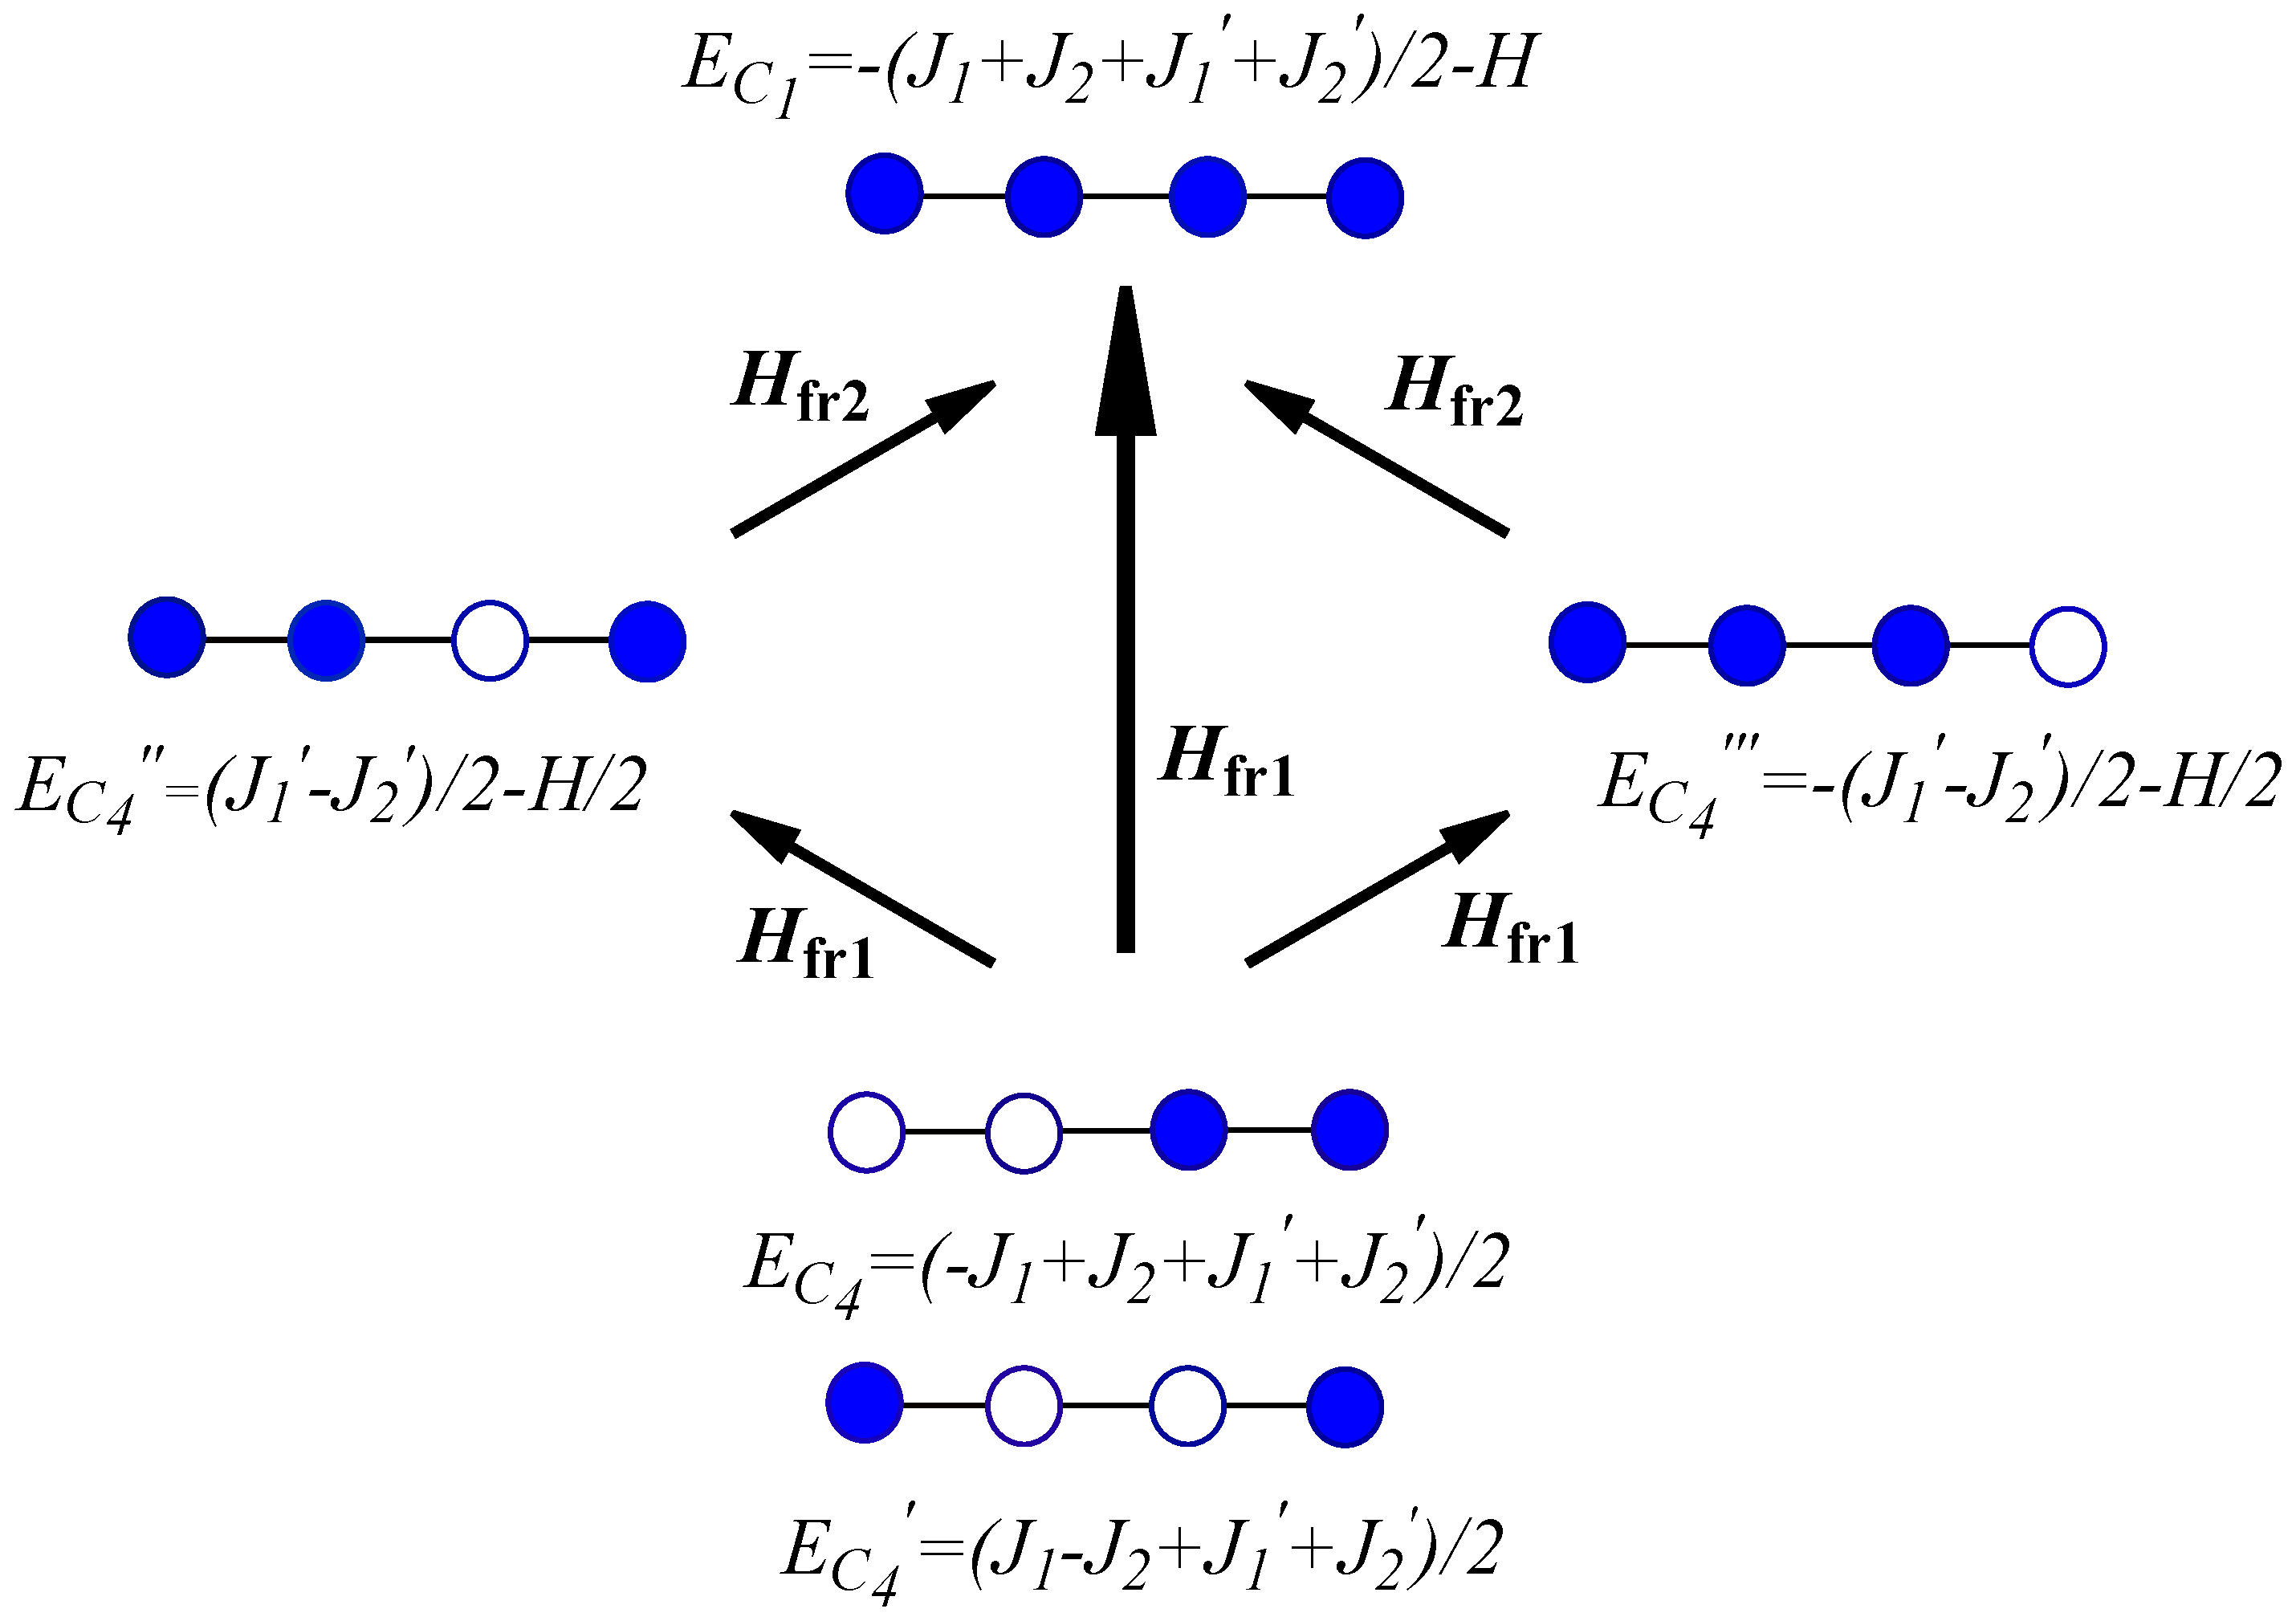
\includegraphics[width=0.7\linewidth]{part2/transGenChain4.eps}}
 	\caption{Конкурирующие взаимодействия $J_1 > 0$, $J_1^{'} < 0$, $J_2 > 0$, $J_2^{'} < 0$ при условии $J_1 = J_2$. Сплошные кружочки --- спин направлен вверх, пустые --- вниз}
 	\label{transGenChain4}
 \end{figure}

\emph{Первое фрустрирующее поле при $R_1 - R_2 \geqslant 1$} (\emph{или $R_1 - R_2 \leqslant -1$}). Происходит переход из фазы учетверения периода трансляции $C_4$ (или $C_4^{'}$) в другую фазу учетверения $C_4^{''}$ (или $C_4^{'''}$) с энтропией \eqref{24} и намагниченностью
\begin{equation}
M_{T\rightarrow 0} = \frac{1}{4\varphi - 2} = 0.2236\dots.
\label{34}
\end{equation}

\emph{Первое фрустрирующее поле при $-1 \leqslant R_1 - R_2 \leqslant 1$}. В этом случае наблюдается переход из фазы учетверения периода трансляции $C_4$ в ферромагнитную конфигурацию $C_1$~\cite{zarubin2019} с энтропией, равной натуральному логарифму наибольшего вещественного корня уравнения $x^4-x^3-1=0$
\begin{equation}
S_{T\rightarrow 0} = \ln \mu = 0.3223\dots,
\label{35}
\end{equation}
\begin{equation}
M_{T\rightarrow 0} = \frac{\mu^4}{\mu^3+4\mu+1} = 0.3967\dots,
\label{36}
\end{equation}
при 
\begin{equation*}
\mu = \frac{1}{4} + \sqrt{\frac{1}{16}\bigg(\frac{1}{2\zeta} + 3\bigg) - \zeta^2} + \zeta ,
\end{equation*}
где $\zeta = \sqrt{1-16\left(\sqrt[3]{(\sqrt{849}+9)/1152}-\sqrt[3]{(\sqrt{849}-9)/1152}\right)}/4$.
Данное математическое сечение пока безымянное.


 \begin{figure}[h]
 	\begin{minipage}{0.47\linewidth}
 		\center{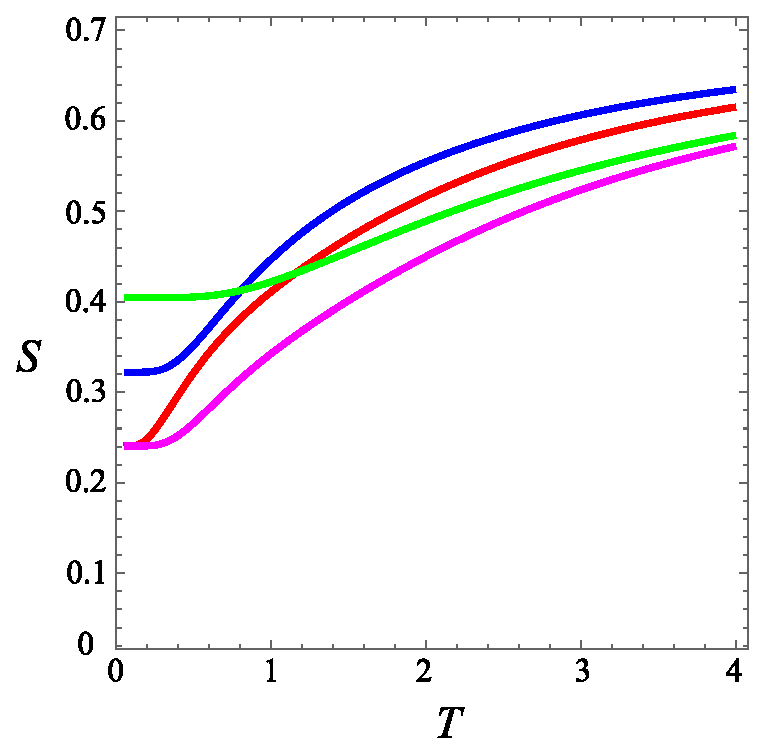
\includegraphics[width=1\linewidth]{part2/entropyGenChain2.eps} \\ а)}
 	\end{minipage}
 	\hfill
 	\begin{minipage}{0.47\linewidth}
 		\center{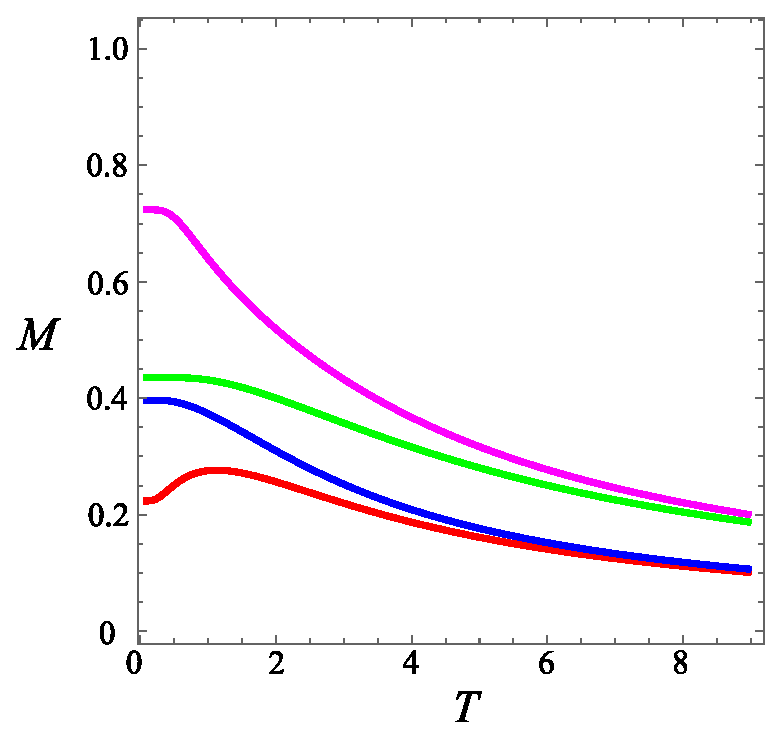
\includegraphics[width=1\linewidth]{part2/magGenChain2.eps} \\ б)}
 	\end{minipage}
 	\caption{Температурные зависимости а) энтропий, б) намагниченностей. Зеленые кривые --- $J_1 = 1$, $J_1^{'} = -2$, $J_2 = 1$, $J_2^{'} = -1$, $H = 2$, красные кривые --- $J_1 = 1$, $J_1^{'} = -2$, $J_2 = -0.5$, $J_2^{'} = -0.5$, $H = 1$, синие кривые --- $J_1 = 1$, $J_1^{'} = -1$, $J_2 = 1$, $J_2^{'} = -1$, $H = 1$, фиолетовые кривые --- $J_1 = 1$, $J_1^{'} = -2$, $J_2 = 1$, $J_2^{'} = -0.5$, $H = 2$}
 	\label{EntAndMagGenChain2}
 \end{figure}

\emph{Первое фрустрирующее поле при $R_1 - R_2 = 1$ или $R_1 - R_2 = -1$}. Происходит переход из фаз с учетверением периода трансляции $C_4$ или $C_4^{'}$ в ферромагнитное упорядочение $C_1$. Энтропия принимает значение натурального логарифма квадратного корня из наибольшего решения уравнения \mbox{$x^3-2x^2-x+1=0$}
\begin{equation}
S_{T\rightarrow 0} = \ln \sqrt{\varkappa} = 0.4048\dots,
\label{37}
\end{equation}
\begin{equation}
M_{T\rightarrow 0} = \frac{\varkappa^2}{2\varkappa^2+2\varkappa-3} = 0.43556\dots,
\label{38}
\end{equation}
где $\varkappa = \Big(2+\sqrt[3]{98/(3\sqrt{3}i+1)}+\sqrt[3]{(21\sqrt{3}i+7)/2}\Big)/3$. Это математическое сечение пока безымянное.

\emph{Второе фрустрирующее поле}. Энтропия определяется из выражения \eqref{24}, а соответствующая намагниченность будет равна выражению \eqref{25}.

Рисунок~\ref{EntAndMagGenChain2} демонстрирует обнаруженные фрустрационные значения энтропий и намагниченностей в данном варианте конкурирующих взаимодействий.

\section{Частные случаи обобщенной модели Изинга на одномерной цепочке в присутствии магнитного поля}

Главным преимуществом обобщенной модели Изинга с несколькими трансляциями в различных направлениях является возможность получения известных видов решеток через предельные переходы. Таким образом, обобщением на произвольное число трансляций можно получить такую решетку, которая будет включать, помимо известных нам решеток, совершенно новые типы структур на плоскости. Рассмотрим данную идею на одномерной цепочке. 

Ниже приведены некоторые частные случаи обобщенной модели Изинга с учетом различных обменных взаимодействий между ближайшими и вторыми соседями, находящихся в магнитном поле. 

\subsection{Единожды декорированная цепочка}

Полагая нулю одно из взаимодействий между вторыми соседями (например, $J_2^{'} = 0$), обобщенная цепочка примет вид, представленный на рисунке~\ref{oneDecorChain}. При $J_1 = J_2$ получим простейший случай декорированной цепочки, а именно, единожды декорированную цепочку~\cite{stephenson1970} с двумя фрустрирующими полями.

 \begin{figure}[h]
 	\center{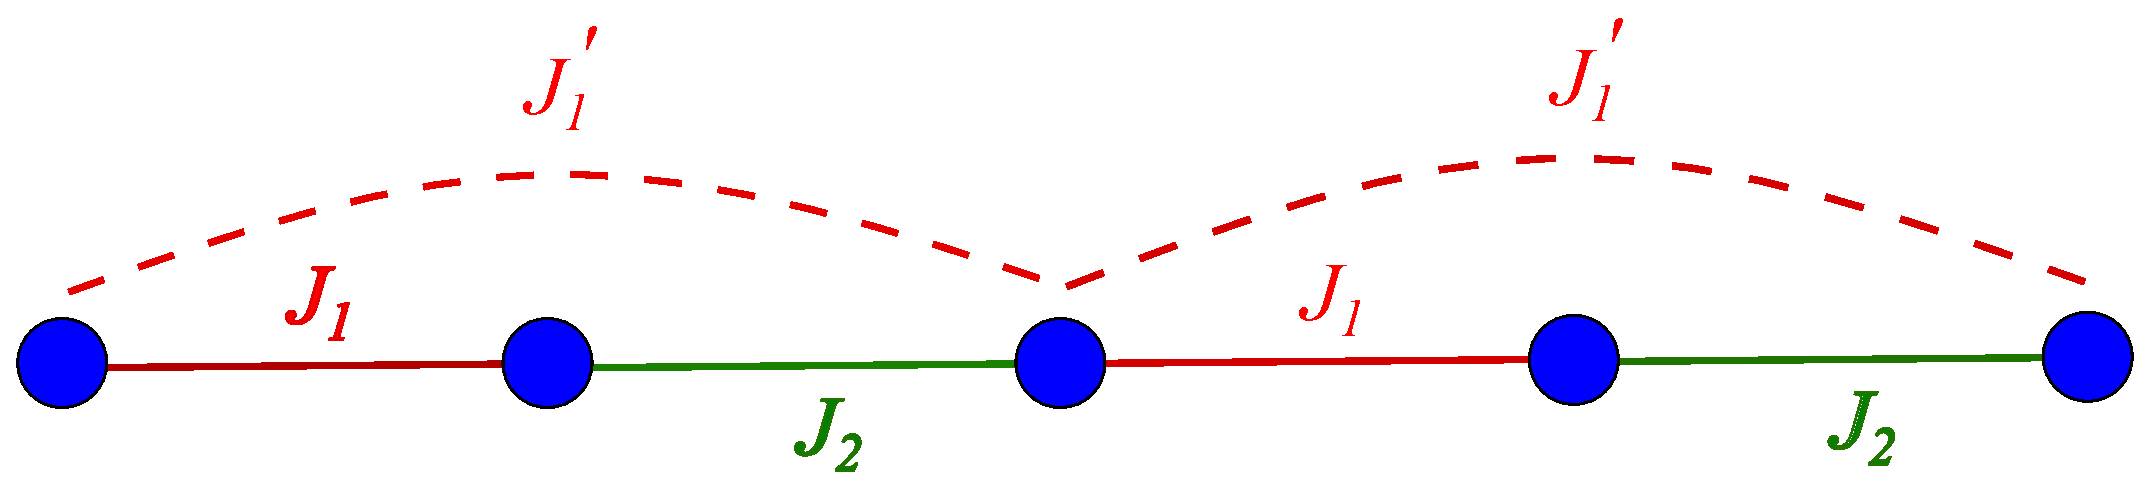
\includegraphics[width=0.8\linewidth]{part2/oneDecorChain.eps}}
 	\caption{Цепочка без взаимодействия $J_2^{'}$. В случае $J_1=J_2$ реализуется случай единожды декорированной цепочки}
 	\label{oneDecorChain}
 \end{figure}

\[
\begin{aligned}
H_{\text{fr}_1}&=
\begin{cases}
-J_{1}-J_{2}, & \text{ при } J_{1}^{'}=0; \\
-J_{1}+2J_{1}^{'}-J_{2}, & \text{ при } 0 \ge J_{1}^{'}\ge J_{2}.
\end{cases}\\
H_{\text{fr}_2}&=-J_{1}-2J_{1}^{'}-J_{2}.
\end{aligned}
\]

\emph{Первое фрустрирующее поле при $J_{1}^{'}=0$}.  Энтропия \eqref{20} с намагниченностью \eqref{25}.

\emph{Первое фрустрирующее поле при $0 \ge J_{1}^{'}\ge J_{2}$}. Энтропия равна натуральному логарифму корня из двух \eqref{32} с намагниченностью \eqref{31}.

\emph{Первое фрустрирующее поле при $J_1^{'} = J_2$ и $J_2^{'} = 0$} (\emph{$J_2^{'} = J_2$ и $J_1^{'} = 0$ аналогично}). Приравнивая взаимодействие между ближайшими соседями к взаимодействию между вторыми соседями, получаем ситуацию при $H_{\text{fr}} = 0$ и с нуль-температурной энтропией равной натуральному логарифму корня из трех 
\begin{equation}
S_{T\rightarrow 0}=\ln \sqrt{3}.
\label{39}
\end{equation}

\emph{Второе фрустрирующее поле}. Энтропия \eqref{24} с намагниченностью \eqref{25}.

\subsection{Набор двух независимых подрешеток}

Довольно любопытный случай получается, если убрать из рассмотрения взаимодействия между ближайшими соседями. Тогда цепочка примет вид, показанный на рисунке~\ref{twoChains}.

 \begin{figure}[h]
 	\center{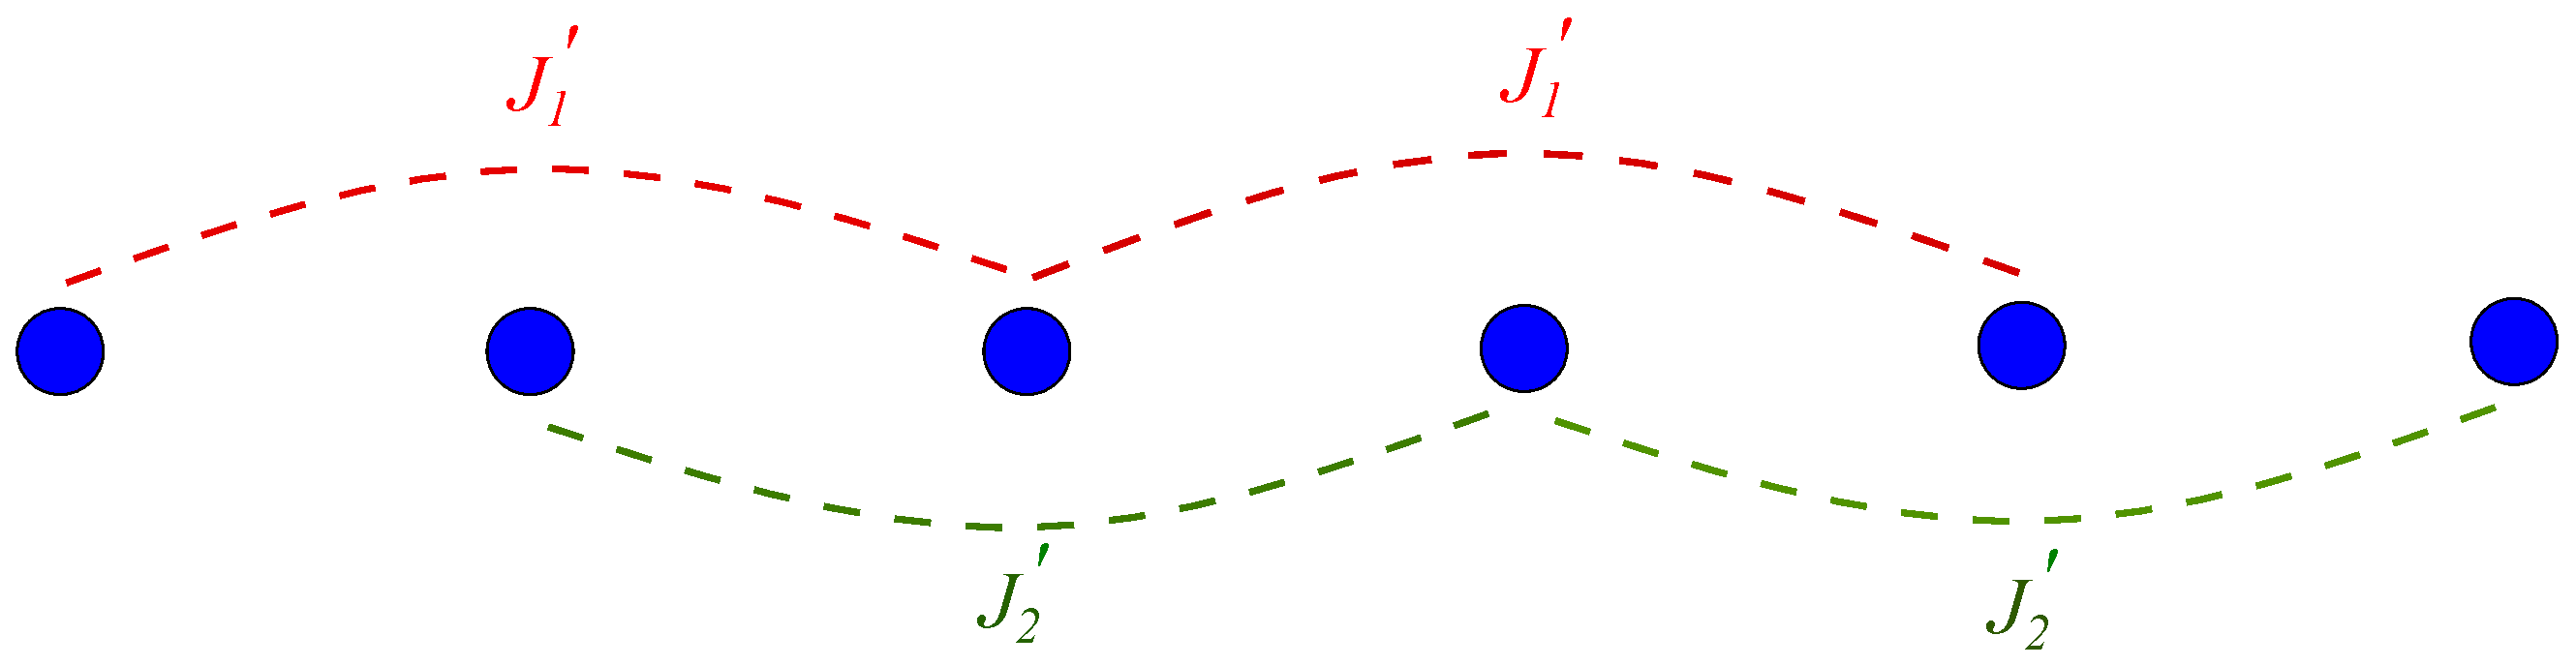
\includegraphics[width=0.8\linewidth]{part2/twoChains.eps}}
 	\caption{Узлы в данной цепочке связаны взаимодействиями только между вторыми соседями, образуя две независимые друг от друга цепочки}
 	\label{twoChains}
 \end{figure}

\[
\begin{aligned}
H_{\text{fr}_1}&=
\begin{cases}
-2J_{1}^{'}, & \text{ при } J_{1}^{'}\leq J_{2}^{'}; \\
-2J_{2}^{'}, & \text{ при } J_{1}^{'}\ge J_{2}^{'}; \\
\end{cases}\\
H_{\text{fr}_2}&=
\begin{cases}
-2J_{2}^{'}, & \text{ при } J_{1}^{'}\leq J_{2}^{'}; \\
-2J_{1}^{'}, & \text{ при } J_{1}^{'}\ge J_{2}^{'}; \\
\end{cases}\\
\end{aligned}
\]

\emph{Первое фрустрирующее поле при $J_{1}^{'}\leq J_{2}^{'}$ или при $J_{1}^{'}\ge J_{2}^{'}$}. Энтропия \eqref{24} с намагниченностью \eqref{34}.

\emph{Первое фрустрирующее поле при $J_{1}^{'} = J_{2}^{'}$}.
Любопытно, что при равенстве взаимодействий можно прийти к результатам, полученным для обычной (не обобщенной) решетки с ближайшими соседями с энтропией \eqref{20} и намагниченностью \eqref{25}.

\emph{Второе фрустрирующее поле}. Энтропия \eqref{24} с намагниченностью \eqref{25}.

\subsection{Цепочка лестничного типа}

Рассмотрим лестничную цепочку (рис.~\ref{ladderChain}). 

\[
\begin{aligned}
H_{\text{fr}_1}&=
\begin{cases}
-J_{2}-2J_{2}^{'}, & \text{ при } R_{2}\leq J_{1}^{'}; \\
-2J_{1}^{'}-J_{2}, & \text{ при } R_{2}\ge J_{1}^{'}.
\end{cases}\\
H_{\text{fr}_2}&=
\begin{cases}
-J_{2}-2J_{1}^{'}, & \text{ при } R_{2}\leq J_{1}^{'}; \\
-2J_{2}^{'}-J_{2}, & \text{ при } R_{2}\ge J_{1}^{'}.
\end{cases}\\
\end{aligned}
\]

 \begin{figure}[h]
 	\center{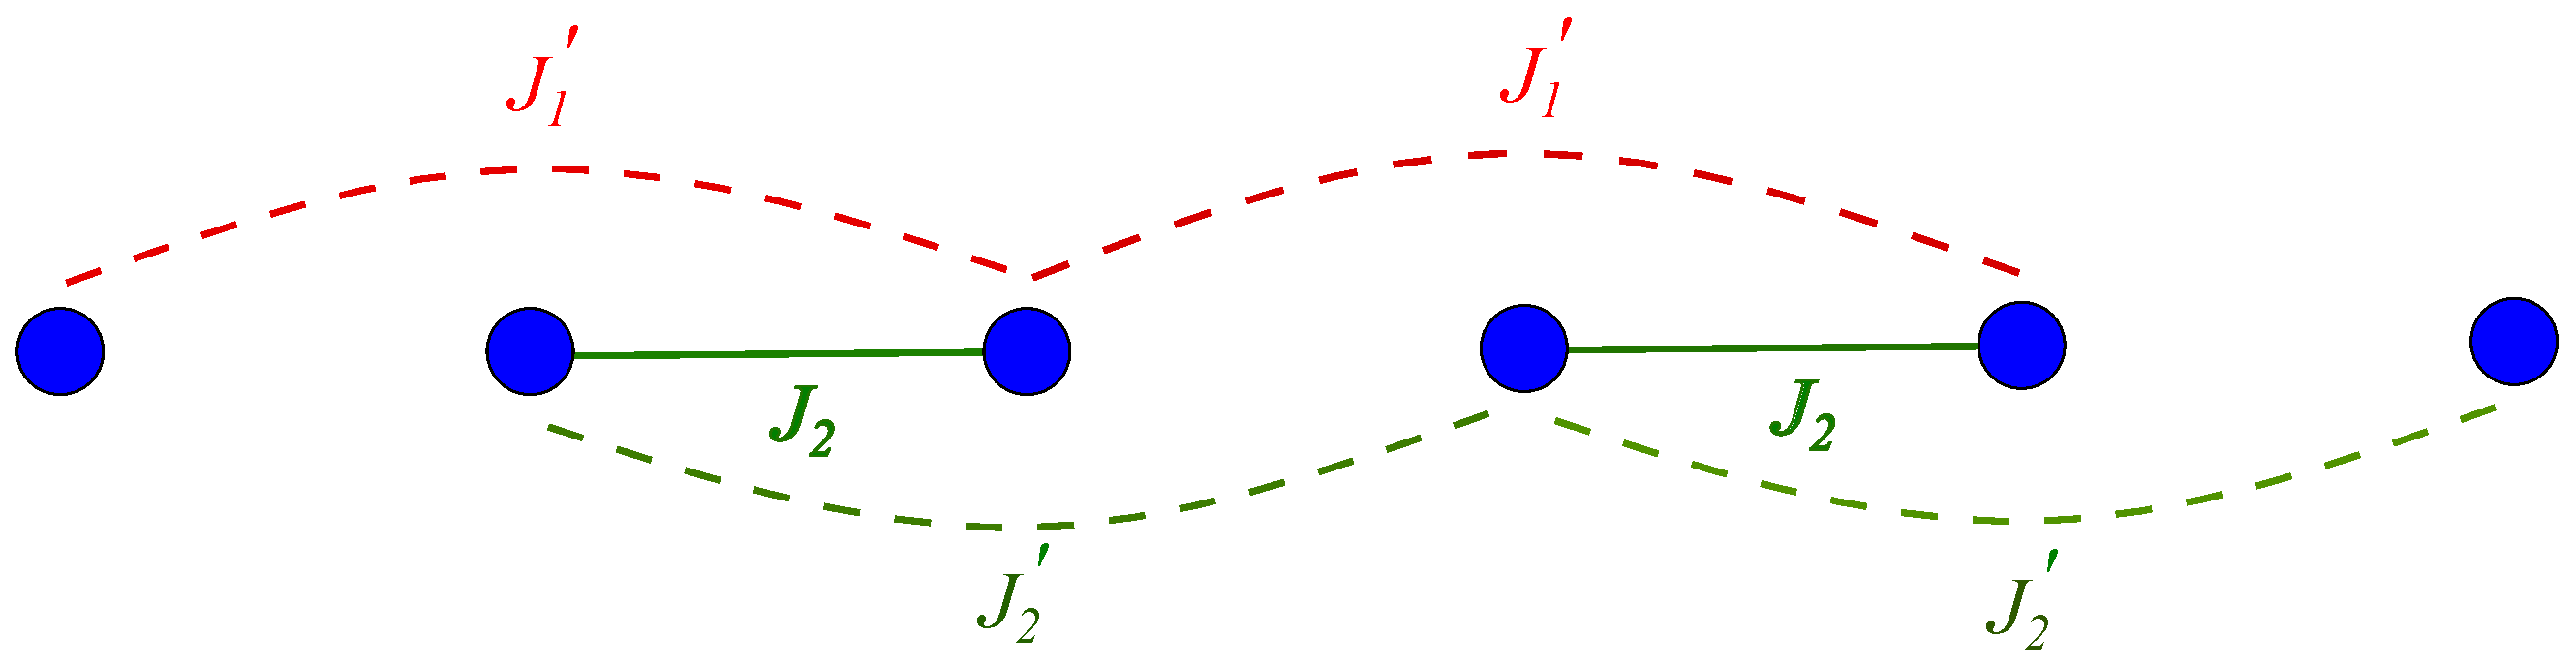
\includegraphics[width=0.8\linewidth]{part2/ladderChain.eps}}
 	\caption{Цепочка лестничного типа}
 	\label{ladderChain}
 \end{figure}

\emph{Первое фрустрирующее поле при $R_{2}\leq J_{1}^{'}$ или при $R_{2}\ge J_{1}^{'}$}. Энтропия \eqref{30} с намагниченностью \eqref{31}.

\emph{Первое фрустрирующее поле при $J_1 = 0$ и $R_2 = J_1^{'}$} (\emph{$J_2 = 0$ и $R_1 = J_2^{'}$ аналогично}). Энтропия равна логарифму квадратного корня наибольшего решения уравнения \mbox{$x^2-x-1=0$}, известного как серебряное сечение
\begin{equation}
S_{T\rightarrow 0} = \ln \sqrt{\delta} = 0.4407\dots, 
\label{40}
\end{equation}
где $\delta = 1 + \sqrt{2}$ --- серебряное сечение, а намагниченность равна $1/2$.

\emph{Второе фрустрирующее поле}. Энтропия \eqref{24} с намагниченностью \eqref{25}.

\subsection{Решетка димеров}

Решетка димеров~\ref{dimerChain} примечательна тем, что ненулевое значение энтропии можно получить при любой величине и знаке взаимодействия в отсутствие магнитного поля. Это значит, что при любом $J_1$ в системе возникают фрустрации --- то есть бесконечное количество конфигураций с одинаковой энергией. В отсутствие магнитного поля имеем $S_{T\rightarrow 0} = \ln(2)/2$, в магнитном поле (при $H = 1$, $J_1 = −1$ или $J_2 = −1$) нуль-температурная энтропия равна $S_{T\rightarrow 0} = \ln(3)/2$.

 \begin{figure}[h]
 	\center{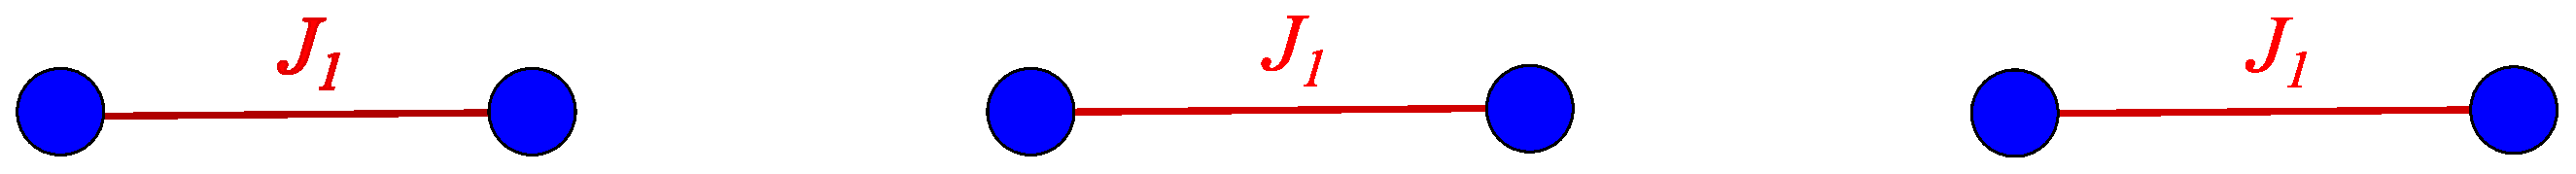
\includegraphics[width=0.8\linewidth]{part2/dimerChain.eps}}
 	\caption{Решетка с ненулевым значением только между ближайшими соседями $J_1$}
 	\label{dimerChain}
 \end{figure}


\section{Общее правило исследования фрустрированных систем}

При исследовании фрустрационных свойств, рассматриваемых в данной модели, обнаружилась любопытная особенность, а именно, при некоторых наборах обменных взаимодействий и некоторых (иногда совпадающих) фрустрационных полях нуль-температурные энтропии и намагниченности могут совпадать. В частности, это имеет место при $J_1=1.0$, $J_1^{'}= -2.0$, $J_2=1.0$, $J_2^{'}= -0.5$, $H=2$, а также при  $J_1= -0.2$, $J_1^{'}= -0.4$, $J_2= -1.0$, $J_2^{'}= -0.2$, $H=2$. 

В этом случае совпадают три наблюдаемых: нуль-температурная энтропия, равная логарифму квадратного корня из золотого сечения \eqref{24}; нуль-температурная намагниченность, равная  золотому сечению, деленному на два золотого сечения минус единица  \eqref{25}, а также фрустрационное поле, равное двум.

 \begin{figure}[h]
	\begin{minipage}{0.47\linewidth}
		\center{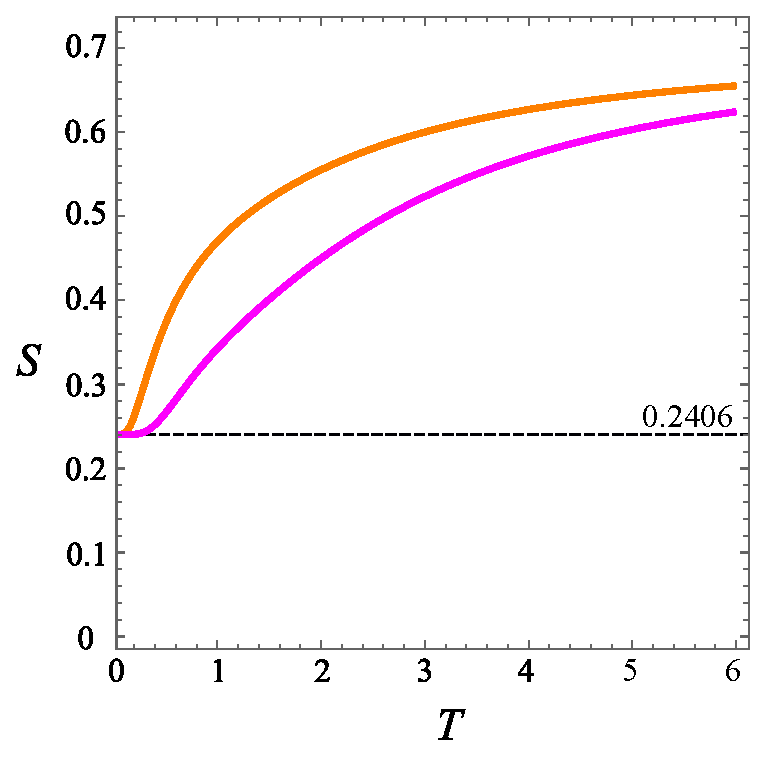
\includegraphics[width=1\linewidth]{part2/entropyResearch.eps} \\ а)}
	\end{minipage}
	\hfill
	\begin{minipage}{0.47\linewidth}
		\center{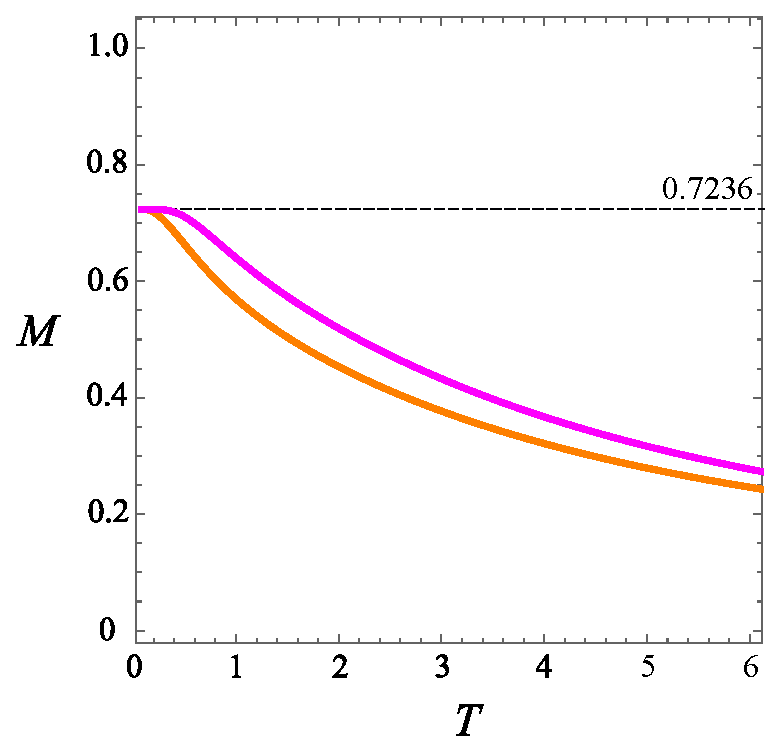
\includegraphics[width=1\linewidth]{part2/magResearch.eps} \\ б)}
	\end{minipage}
	\vfill
	\begin{minipage}{0.47\linewidth}
		\center{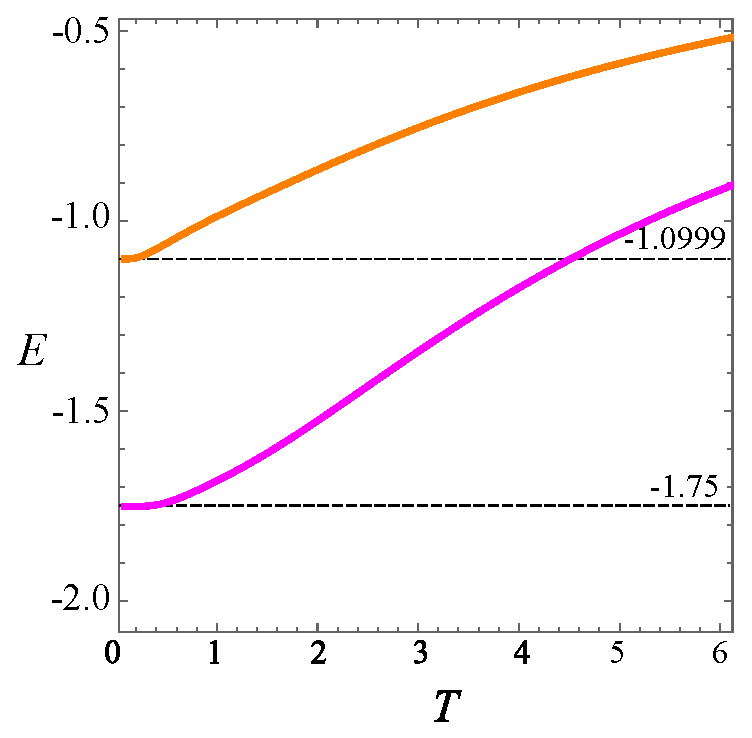
\includegraphics[width=1\linewidth]{part2/energyResearch.eps} \\ в)}
	\end{minipage}
	\hfill
	\begin{minipage}{0.47\linewidth}
		\center{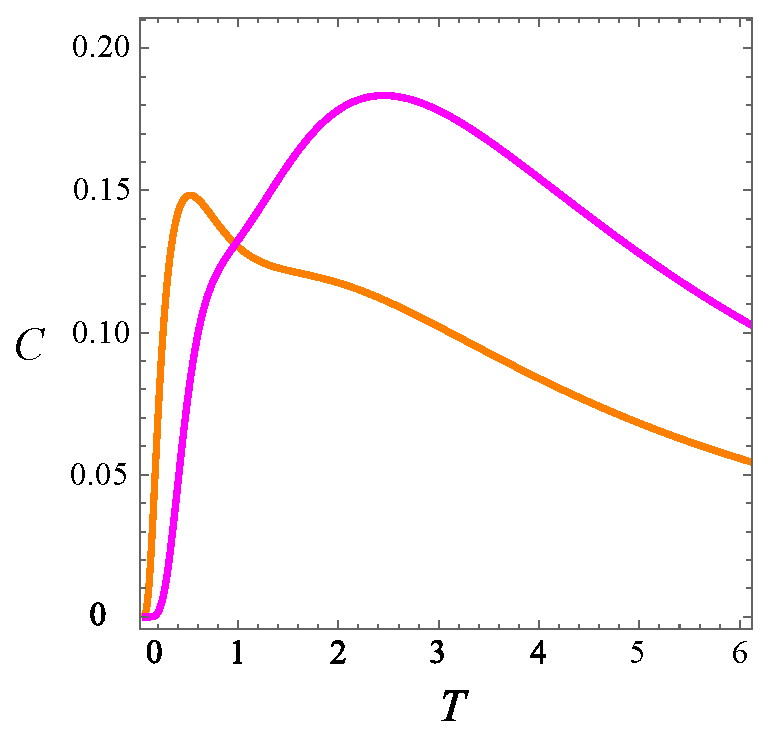
\includegraphics[width=1\linewidth]{part2/heatResearch.eps} \\ г)}	
	\end{minipage}
	\caption{Температурные зависимости а) энтропий, б) намагниченностей, в)  внутренних энергий, г) теплоемкостей. Фиолетовые кривые --- $J_1=1.0$, $J_1^{'}= -2.0$, $J_2=1.0$, $J_2^{'}= -0.5$, $H=2$, оранжевые кривые --- $J_1= -0.2$, $J_1^{'}= -0.4$, $J_2= -1.0$, $J_2^{'}= -0.2$, $H=2$}
	\label{research}
\end{figure}

Таким образом, создается впечатление, что поведение системы (по крайней мере, в основном состоянии) одинаково при обменных взаимодействиях, \emph{разных как по величине, так и по знаку}. Ложность этого впечатления доказывается при дополнительном исследовании других наблюдаемых, а именно теплоемкости и особенно внутренней энергии, \emph{существенно разной} даже в основном состоянии (см. рис.~\ref{research}). Отсюда следует важный вывод о том, что получение истинного поведения системы может быть достигнуто только при комплексном исследовании, а исследование ограниченного числа наблюдаемых приводит к ошибочным результатам.

\section{Выводы по главе}

Благодаря выведенной обобщенной трансфер-матрице Крамерса--Ваннье появилась возможность рассматривать решетки с наличием большего количества конкурирующих взаимодействий, что, в свою очередь, позволит лучше понять особенности фрустрированных спиновых систем

Кроме того, обобщение модели Изинга можно рассматривать не только при учете ближайших и вторых соседей, но и при участии третьих~\cite{zarubin2020}, четвертых и других дальних соседей, как при наличии магнитного поля, так и в его отсутствие.

Следует отметить, что обобщение на множество трансляций решетки можно реализовать и в других статистических моделях (например, в моделях Поттса) на различных вариантах решеток~\cite{proshkinThesis, kassan-ogly2000_1, kassan-ogly2000_2, proshkin2015, kassan-ogly2015}.

Также, алгоритм построения обобщенной модели Изинга позволяет ввести квантовую обобщенную модель Изинга (с произвольным значением спина)~\cite{proshkin2016, proshkin2018}.

Результаты, описанные в этой главе, опубликованы автором в работах~\cite{confbib1, confbib2, vakbib1, vakbib3, confbib6, scbib1}.

\FloatBarrier
